\def \currentAuthor {Das Projektteam} %so kann jederzeit der Autor geändert werden -> wird in der Fusszeile angezeigt.

\chapter*{Einleitende Bemerkungen}

\chapter*{Notationen}
Beschreibung wie Code, Hinweise, Zitate etc. formatiert werden  


\chapter{Projektmanagement}
%todo: Projektmanagementscheiße bullshitten
\section{Metainformationen}
\subsection{Team}
\subsection{Betreuer}
\subsection{Partner}
\subsection{Ansprechpartner}
\section{Vorerhebungen}
\subsection{Projektzieleplan}


\newpage
\subsection{Projektumfeld}
\begin{itemize}
	\item Identifikation der Stakeholder
	\item Charakterisierung der Stakeholder
	\item Maßnahmen
	\item Grafische Darstellung des Umfeldes
\end{itemize}
\subsection{Risikoanalyse}
\subsubsection{Risikoidentifikation}
Folgende Risiken können während der Projektdurchführung erwartet werden:
\begin{itemize}
	\item[\textbf{R1}] Projektmitglied steig aus dem Projekt aus.
	\item[\textbf{R2}] Projektpartner stellt seine Kooperation ein.
	\item[\textbf{R3}] Projektpartner ändert seine Anforderungen.
	\item[\textbf{R4}] Termine können nicht eingehalten werden.
	\item[\textbf{R5}] Anforderungen werden nicht erreicht.			
\end{itemize}

\subsubsection{Bewertung und Behandlung}
Die aufgelisteten Risiken werden nach Auswirkung und Eintrittswahrscheinlichkeit bewertet.
Je höher die Zahl in der Tabelle, desto höher ist die Auswirkung bzw. Einwirkung.
\begin{table}[h]
	\begin{tabular}{l|c|c}
		\textbf{Risiko}                           & \multicolumn{1}{l|}{\textbf{Wahrscheinlichkeit}} & \multicolumn{1}{l}{\textbf{Auswirkung}} \\ \hline
		\textbf{R1} Ausstieg Projektmitglied                  & 3                                                & 10                                      \\
		\textbf{R2} Projektpartner stellt Kooperation ein     & 2                                                & 10                                      \\
		\textbf{R3} Projektpartner ändert seine Anforderungen & 4                                                & 7                                       \\
		\textbf{R4} Termine können nicht eingehalten werden   & 3                                                & 6                                       \\
		\textbf{R5} Anforderungen werden nicht erreicht       & 2                                                & 8                                      
	\end{tabular}
	\caption{Analyse Einwirkung \& Auswirkung}
	\label{Abb_Einwirkung_Auswirkung}
\end{table}
\newpage

\subsubsection{Risikomatrix}
\begin{figure}[h]
	\centering
	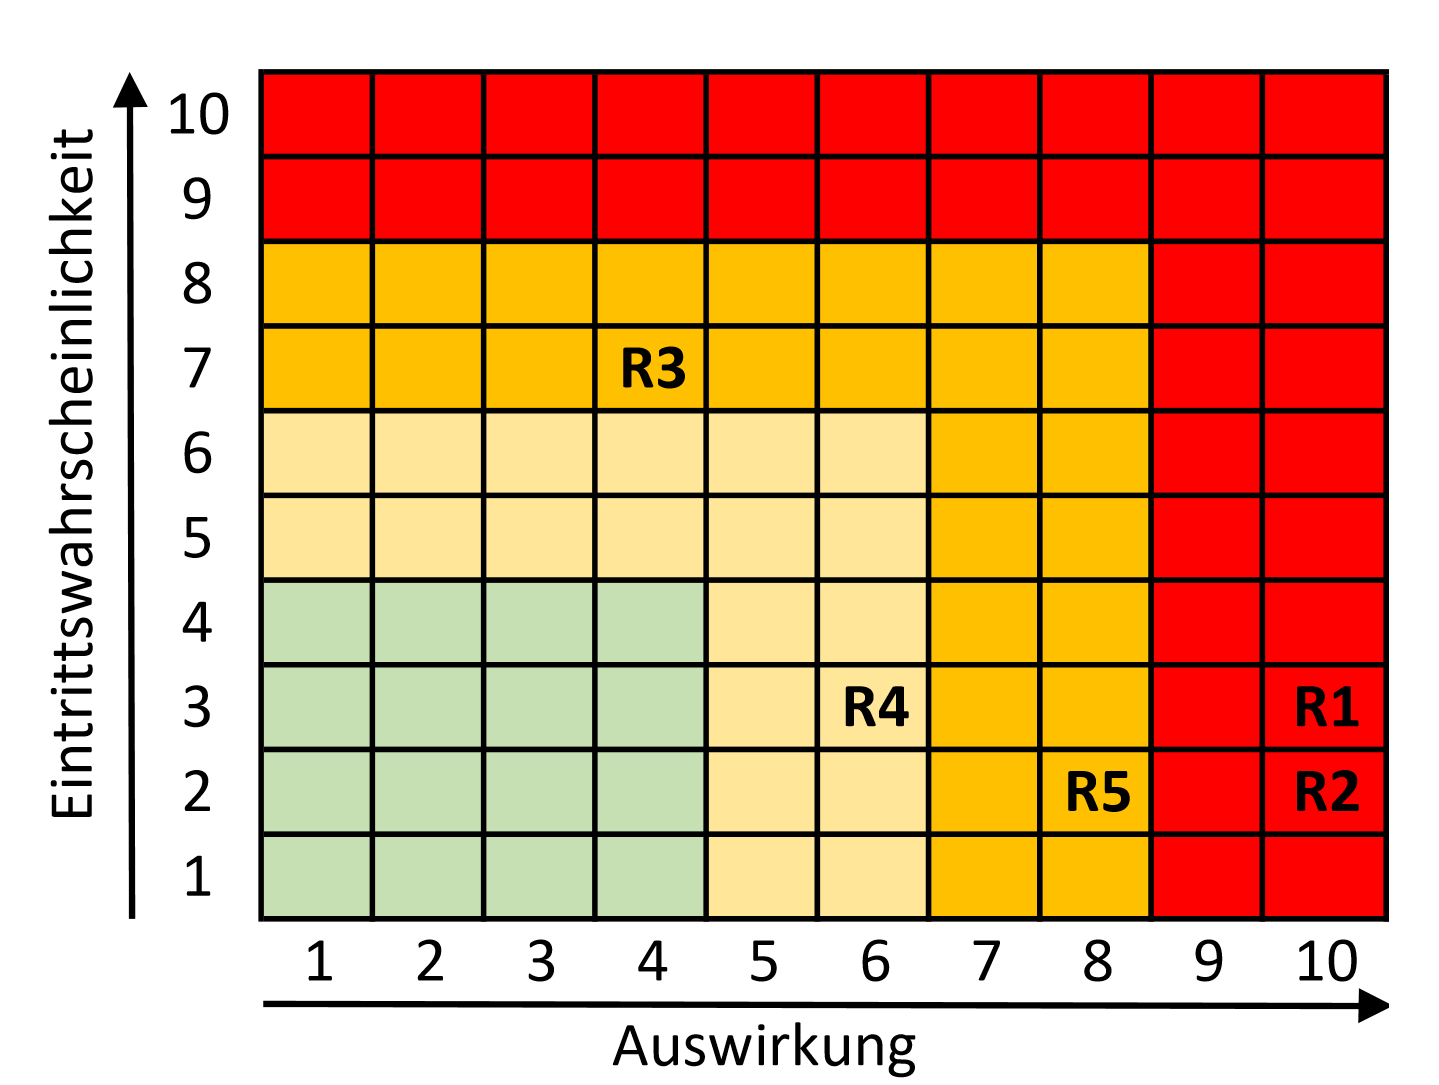
\includegraphics[scale=0.6]{figures/matrix.png}
	\caption{Risikomatrix}
	\label{Abb_Risikomatrix}
\end{figure}


\newpage
\section{Pflichtenheft}
\subsection{Zielbestimmung}
\section{IST Zustand}
IT-ManagerInnen an Tirols Schulen können Probleme mit der Infrastruktur melden und Anfragen zur Beschaffung von Ressourcen/Komponenten stellen.
\\
Sie können den Bearbeitungsverlauf ihrer Tickets beobachten. SystembetreuerInnen empfangen die Tickets der IT-ManagerInnen, welche sich in ihrem Cluster befinden. SystembetreuerInnen bearbeiten die Tickets und antworten auf die Anfragen.

\begin{figure}[h]
	\centering
	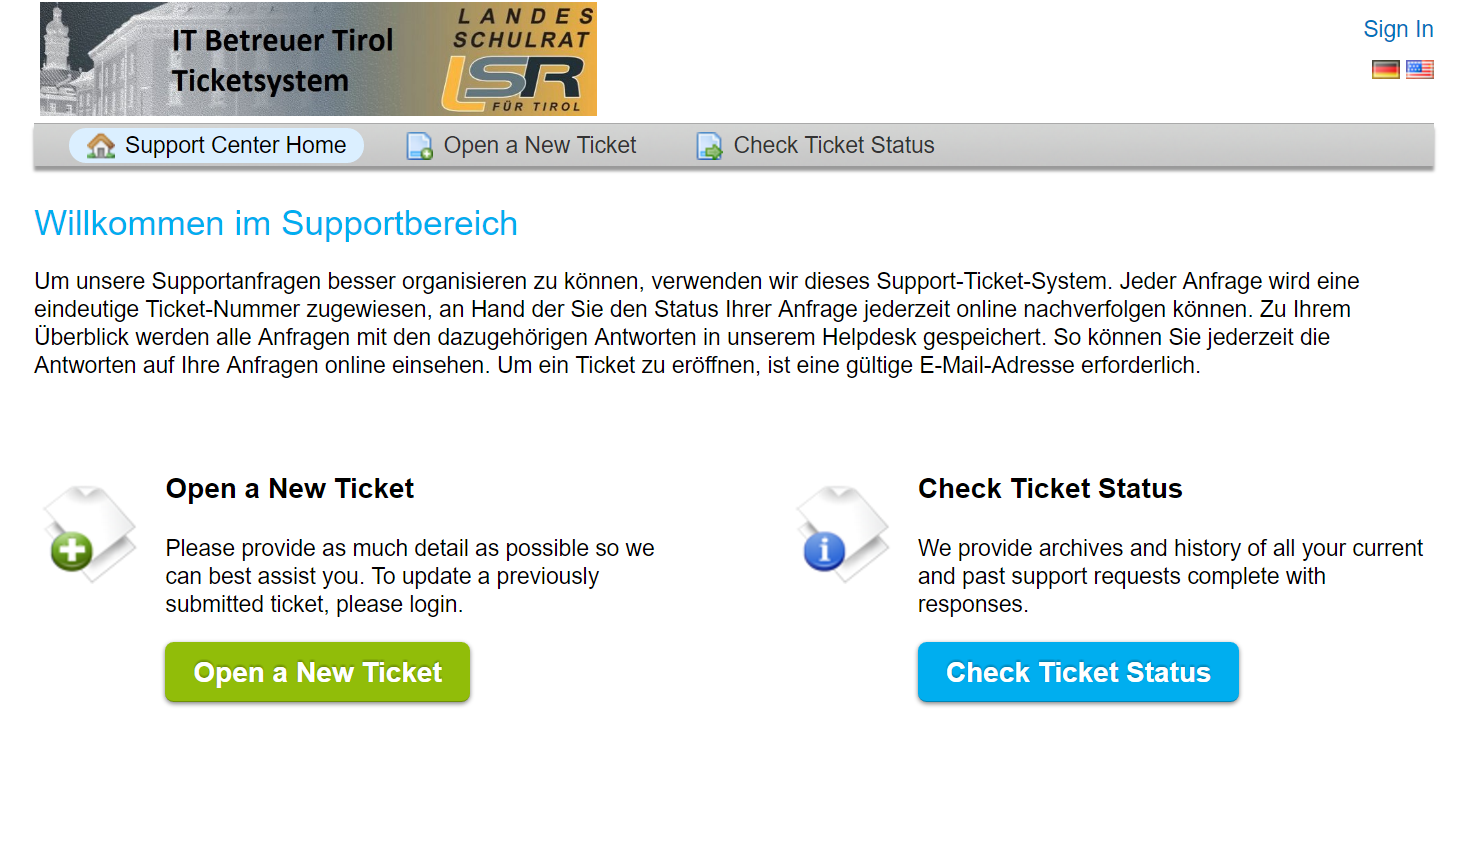
\includegraphics[scale=0.725]{figures/Ist_Login.png}
	\caption{IST-Zustand OS-Ticket}
	\label{Abb_IST-Zustand}
\end{figure}
\noindent Die Benutzerschnittstelle ist derzeit nur auf die Benutzung mit großen Bildschirmen (ab 1024 Pixel Bildschirmbreite) ausgelegt. Sie kann sich nicht an kleinere Formate (Smartphone, etc.) anpassen.

\section{SOLL Zustand}
Bessere Usability soll mit Hilfe von Mobile-First Orientierung auf Basis von Bootstrap erreicht und wenn möglich die Ticketerstellung vereinfacht werden.
\\
Das Backend soll die Aufteilung in mehrere hierarchische Organisationseinheiten ermöglichen und eine Erweiterung von Landesebene auf Bundesebene zulassen. Des Weiteren gilt es, den AnwenderInnen den Ticketingprozess intuitiver zu gestalten.

\subsection{SMART}
\begin{description}
	\item[S] Spezifisch\newline
	Systembetreuer und IT-Manager können Support- und Beschaffungsanfragen mit Hilfe des Ticketsystems abwickeln.
	\item[M] Messbar\newline
	Systembetreuer empfangen die Tickets und kümmern sich um die Probleme. Die Schulen werden in Cluster eingeteilt und von Systembetreuern verwaltet. 
	\item[A] Attraktiv\newline
	Die Plattform muss auf jedem Endgerät verfügbar sein (Responsive Design). Das Absetzen und Ansehen von Tickets soll vereinfacht werden, die Plattform bietet einige Funktionen die für das System relevant sind.
	\item[R] Realisierbar\newline
	Zum Realisieren wird eine Testumgebung von Seiten des Betreuers zur Verfügung gestellt. Das Responsive Design wird mithilfe eines Framework (Bootstrap) realisiert.
	\item[T] Terminisierbar\newline
	Im Juni 2017 wird das Projekt abgeschlossen und eine technische Dokumentation des Projekts liegt vor.
\end{description}


\subsection{Produkteinsatz und Umgebung}
%--------------------------------
%todo: Anwender des Systems beschreiben (steht auch so in der Vorlage)
%--------------------------------
\subsection{Projektumfeldanalyse}
\subsubsection{Einflussfaktoren}
Das Projekt wurde durch den Landesschulrat Tirol in Auftrag gegeben. Die Ansprechperson, Herr Helmut Hammerl, informiert uns über den IST und SOLL-Zustand der Plattform und unterstützt das Projekt mit Ideen und Hilfestellungen bei Problemstellungen.
\\
Des Weiteren beeinflussen die Anwender (IT-Manager) und die Systembetreuer der Plattform das Projektresultat. Da auf die Anwenderfreundlichkeit viel Wert gelegt wird, spielen diese Faktoren eine wirkliche Rolle.
\\
Die Projektbetreuer Stefan Stolz und Alexander Scharmer sind für auftretende Fragen, bezüglich Problemstellungen die während des Projekts auftreten können, enorm einflussreich.
\newpage
\subsection{Stakeholder}
\subsubsection{Stakeholder Identifizieren}
\begin{table}[h]
	\centering
	\begin{tabular}{|lll|}
		\hline
		Stakeholder          & Einfluss &  Konfliktpotential      \\ \hline                         
		Mag. Helmut Hammerle & 3         & 0                  \\ 
		Dr. Stefan Walch     & 2         & 0                  \\
		Stefan Stolz         & 1         & +                  \\ 
		Alexander Scharmer   & 1         & +                  \\ 
		Michael Gamper       & 0         & 0                  \\ 
		LSI DI Anton Lendl   & 3         & 0                  \\ 
		Team Mitglieder      & 2         & 0                   \\ \hline			
	\end{tabular}
	\caption{Stakeholder Identifikation}
	\label{Tbl_Stakeholder_Identifikation}
\end{table}


\subsubsection{Stakehnolder Klassifizieren}	

%todo: Formatierung der Tabelle
\begin{table}[h]
	\centering
	\begin{tabular}{|lll|}
		\hline
		Stakeholder          & Risiken durch Stakeholder                        & Strategien                                            \\ \hline
		Mag. Helmut Hammerle & Ändern der Ansprüche          & Unterschriebenes Pflichtenheft  \\
		Dr. Stefan Walch      & Nicht bestätigen des Projektantrages             & Durchdachter Projektantrag                            \\
		Stefan Stolz         & falsche Informationen, kein Interesse & regelmäßiges Treffen             \\
		Alexander Scharmer   & falsche Informationen, kein Interesse & regelmäßiges Treffen              \\
		Michael Gamper       & Nicht bestätigen des Projektantrages             & Durchdachter Projektantrag                            \\
		LSI DI Anton Lendl   & Nicht bestätigen des Projektantrages             & Durchdachter Projektantrag                            \\
		Team Mitglieder      & Mangelnde Motivation                             & Faire Arbeitsverteilung           \\ \hline			
	\end{tabular}
	\caption{Stakehodler Klassifikation}
	\label{Tbl_Stakeholder_Klassifikation}
\end{table}


\subsection{Funktionalitäten}
\subsection{Muss Anforderungen}
IT-ManagerInnen und Systembetreuer müssen sich unter itsys-tirol.at, einem Portal des Landesschulrates, basierend auf OSticket anmelden können. Des Weiteren sollen die Schulen selbst bestimmen, wer einen Zugang zum Portal erhalten soll, um Tickets erstellen zu können.
\\
Die angemeldeten IT-ManagerInnen müssen Probleme mit der Infrastruktur melden können und Anfragen zur Beschaffung von Ressourcen bzw. Komponenten einreichen können.
\\
SystembetreuerInnen müssen die Tickets der IT-ManagerInnen empfangen, welche sich in ihrem Cluster befinden. Die eingereichten Tickets sollen von den Systembetreuern bearbeitet werden können.

\subsection{Soll Anforderungen}
Es soll eine neue Weboberfläche entwickelt werden, die auf dem HTML \& CSS Framework Bootstrap basiert. Dieses soll sich auf Einfachheit in der Anwendung und Benutzerfreundlichkeit fokussieren. Die Latenzzeit sollte so niedrig wie möglich gehalten werden um ein Reibungsloses Arbeiten zu ermöglichen.

%todo: Testfälle sind furchtbar und müssen generell nocheinmal überarbeitet werden
\subsection{Testszenarien und Testfälle}
Die Testfälle in unserem Projekt beziehen sich auf das Ticketingsystem OSTicket.

\section{Testfälle}
\subsection{Testfall A}
\begin{itemize}
	\item \textbf{Beschreibung:} Ein IT-Manager möchte ein Ticket erstellen.
	\item \textbf{Vorbedingung:} Der User benötigt ein internetfähiges Gerät und muss im Portal eingeloggt sein.
	\item \textbf{Aktion:} Der Benutzer wählt den Tab "Neues Ticket" und füllt die notwendigen Felder aus.
	\item \textbf{Soll-Reaktion:} Das System setzt das Ticket für den zuständigen Systembetreuer sichtbar.
\end{itemize}
Tester:
\\M
Datum:

\subsection{Testfall B}
\begin{itemize}
	\item \textbf{Beschreibung:} Ein Systembetreuer möchte ein Ticket bearbeiten.
	\item \textbf{Vorbedingung:} Der Systembetreuer benötigt ein internetfähiges Gerät und muss im Portal eingeloggt sein.
	\item \textbf{Aktion:} Der Systembetreuer wählt den Tab "Meine Tickets" und wählt ein Ticket aus das Bearbeitet werden muss. Durch die Beschreibung des Tickets, weiß der Systembetreuer über die Problemstellung Bescheid und kann dementsprechend handeln.
	\item \textbf{Soll-Reaktion:} Der Systembetreuer kann sich um die Problemstellung kümmern und das Ticket nach erfolgreicher Bearbeitung wieder schließen.
\end{itemize}
Tester:
\\
Datum:

\subsection{Testfall C}
\begin{itemize}
	\item \textbf{Beschreibung:} Ein Anwender möchte ein bestimmtes Ticket suchen und dieses begutachten. 
	\item \textbf{Vorbedingung:} Der Anwender benötigt ein internetfähiges Gerät und muss im Portal eingeloggt sein.
	\item \textbf{Aktion:} Der Anwender gibt im Suchfeld ein Stichwort ein nach dem er suchen möchte. 
	\item \textbf{Soll-Reaktion:} Das gesuchte Ticket soll angezeigt werden.
\end{itemize}
Tester:
\\
Datum:



\subsection{Liefervereinbarung}
\begin{itemize}
	\item Lieferumfang
	\item Modus
	\item Verteilung(Deployment)
\end{itemize}

%todo: viel Bullshitten
\section{Planung}
\subsection{Projektstrukturplan}
\subsection{Meilensteine}
\subsection{Gant-Chart}
\subsection{Abnahmekriterien}
\subsection{Pläne zur Evaluierung}
\subsection{Ergänzungen und zu klärende Punkte}

\chapter{Produktvorstellung}
In diesem Kapitel wird das Softwaresystem \getOst\ dokumentiert bzw. vorgestellt sowie dessen Eignung für die Anforderungen des Projektauftraggebers bearbeitet. Die im Zuge des Projektes geplante Modifikation von \getOst\ wird behandelt und es wird erläutert, warum diese nicht in einem angemessenen Rahmen durchführbar ist. Des Weiteren werden die Ansätze und unternommenen Schritte um das ursprüngliche Projektziel zu erreichen, dargestellt.

\section{Realisierbarkeit mit \getOst}
\getOst\ hat sich als umfangreicher herausgestellt wie zu Beginn des Projekts angenommen wurde. Nach Ausarbeitung des konzeptuellen Zieles des Projektes erfolgte eine lange Phase der Evaluation, Einarbeitung und Dokumentation von \getOst. Nach ca. 30 Stunden dieser (viel zu langen) Phase, in der die Komplexität und Schwerfälligkeit des Systems \getOst\ sich nicht bezwingen lassen wollte. Die Anzahl der Dateien setzt sich folgendermaßen zusammen:

\begin{table}
	\centering
	\begin{tabular}{|c|c|}
		\hline 
		Dateityp	& Dateianzahl \\ 
		\hline 
		.php		& 414 \\ 
		\hline 
		.css		& 15 \\ 
		\hline 
		.less		& 9 \\ 
		\hline 
		.sql		& 61 \\ 
		\hline 
		.html		& 1 \\ 
		\hline
		\hline 
		Gesamt		& 500 \\ 
		\hline 
	\end{tabular}

	\label{tbl_ost_dateianzahl}
	\caption{Anzahl der unterschiedlichen Dateitypen in \getOst}
\end{table}

Ein weiteres Hindernis ergibt sich durch den Mangel an einer auch nur annähernd aktuellen Dokumentation des laufend erweiterten und angepassten \getOst.

Damit ist \getOst\ nicht nur wegen der fehlenden Dokumentation kaum zu bändigen, sondern aufgrund seines ständigen Wachstums zu \glqq crufty\grqq , um mit sinvollem Aufwand angepasst zu werden:

\blockcquote{cmdlinestephenson}{
	 In the jargon of hackers\footnote{Der Kontext, aus dem dieses Zitat stammt (die IT-Welt um 1999), verwendet den Begriff \glqq Hacker\grqq\ auch für Personen, die Pionierarbeit in der Softwareentwicklung leisteten.}, it is called
	\glqq cruft.\grqq\ An operating system that has many, many layers of it is described as \glqq crufty.\grqq \\
	Hackers hate to do things twice, but when they see something crufty, their first impulse
	is to rip it out, throw it away, and start anew.
	[...]
	Like an upgrade to an old building, cruft always seems like a good idea when the first layers of it go on – just routine maintenance, sound prudent management. This is especially true if (as it were) you never look into the cellar, or behind the drywall. But if you are a hacker who spends all his time looking at it from that point of view, cruft is fundamentally disgusting, and you can’t avoid wanting to go after it with a crowbar. Or, better yet, simply walk out of the building – let the Leaning Tower of Pisa fall over – and go make a new one THAT DOESN’T LEAN.
}

Um die Realisierbarkeit zu veranschaulichen nun einige Codeauszüge aus OSTicket.
\newpage
\subsection{Codeausschnitte osTicket}
%todo: Zeilennummerierung anpassen (18-31)
\begin{lstlisting}[language=PHP, caption=main.inc.php]
#Disable direct access.
if(isset($_SERVER['SCRIPT_NAME'])
&& !strcasecmp(basename($_SERVER['SCRIPT_NAME'])
,basename(__FILE__)))
die('kwaheri rafiki!');

require('bootstrap.php');
Bootstrap::loadConfig();
Bootstrap::defineTables(TABLE_PREFIX);
Bootstrap::i18n_prep();
Bootstrap::loadCode();
Bootstrap::connect();

#Global override
$_SERVER['REMOTE_ADDR'] = osTicket::get_client_ip();

\end{lstlisting}
%todo: Zitate (Codezitate des Programmierers, Netzer fragen)
In diesem Codeauszug wird die Lesbarkeit des Codes sehr gut veranschaulicht, der Aufruf von elf statischen Funktionen ohne Dokumentation erschwert die Erweiterbarkeit um ein vielfaches. Der einzige Kommentar des Programmierers \textit{Don't Monkey around with} it ist weder aussagekräftig noch hilfreich.
\newpage
%todo: Zeilennummerierung anpassen (51-65)
\begin{lstlisting}[language=PHP, caption=pwreset.php]
$inc = 'register.confirmed.inc.php';
$acct->confirm();
// FIXME: The account has to be uncached in order for the lookup
// in the ::processSignOn to detect the confirmation
ModelInstanceManager::uncache($acct);
// Log the user in
if ($client = UserAuthenticationBackend::processSignOn($errors)) {
if ($acct->hasPassword() && !$acct->get('backend')) {
$acct->cancelResetTokens();
}
// No password setup yet -- force one to be created
else {
$_SESSION['_client']['reset-token'] = $_GET['token'];
$acct->forcePasswdReset();
}
\end{lstlisting}
Auch in der Datei \textit{pwreset.php} ist nur eine sehr dürftige Dokumentation vorzufinden. Es sind lediglich vier Inhaltslose Kommentare wie \textit{makes includes happy} und ein \textit{FIXME} vorzufinden. Diese geben keinerlei Aufschluss über die Funktionalität und Zuständigkeit des Codes.
\newpage
%todo: Zeilennummerierung anpassen (16-23)
\begin{lstlisting}[language=PHP, caption=offline.php]
require_once('client.inc.php');
if(is_object($ost) && $ost->isSystemOnline()) {
@header('Location: index.php'); //Redirect if the system is online.
include('index.php');
exit;
}
$nav=null;
require(CLIENTINC_DIR.'header.inc.php');
\end{lstlisting}
Der einzige Kommentar des Programmierers \textit{modify to fit your needs} erschwert die Lesbarkeit dieser Datei enorm.

%todo: Zeilennummerierung anpassen (38-48)
\begin{lstlisting}[language=PHP, caption=client.inc.php]
/* include what is needed on client stuff */
require_once(INCLUDE_DIR.'class.client.php');
require_once(INCLUDE_DIR.'class.ticket.php');
require_once(INCLUDE_DIR.'class.dept.php');

//clear some vars
$errors=array();
$msg='';
$nav=null;
//Make sure the user is valid..before doing anything else.
$thisclient = UserAuthenticationBackend::getUser();
\end{lstlisting}
In der Datei client.inc.php wird lediglich dokumentiert, dass diese Datei in jeder client page inkludiert wird. Der Code in dieser Datei besteht hauptsächlich aus statischen Funktionsaufrufen.

\subsection{Evaluation Katak}
In progress
\subsection{Evaluation OSTicky}
in progress



%----------------------------------------------
\section{Systemdokumentation}
%todo: Systemdokumentation aus SYP hinzufügen, ist jedoch nicht ganz so einfach da Probleme mit Packages auftreten 

\documentclass[10pt,a4paper]{article}
\usepackage[utf8]{inputenc}
\usepackage{amsmath}
\usepackage{amsfonts}
\usepackage{amssymb}
\usepackage{graphicx}
\usepackage[left=30mm, right=20mm, top=30mm, bottom=30mm]{geometry}
\usepackage[german]{babel}
\usepackage{graphicx,array}
\usepackage{fancyhdr}
\usepackage{setspace}
\usepackage{wrapfig}


%#######################


	\section{Verwendete Technologie}
	\subsection{OSTicket}
	OSTicket ist ein weit verbreitetes, quelloffenes Ticketingsystem. Es verfügt über eine zentrale MySQL-Datenbank und ein Multi-User Web Interface. Dieses Webinterface gilt es im Zuge dieses Projektes so aufzubereiten, dass es neben den üblichen Auflösungen von Desktop- und Laptopbildschirmen auch Mobile Displays wie die von Smartphones oder Tablets unterstützt.
	
	\begin{wrapfigure}{r}{0.4\textwidth}
		\vspace{-1cm}
		\begin{center}
		\caption{OSTicket Logo}
		\vspace{.5cm}
		
\includegraphics[scale=.7]{figures/icon_osticket.png}
		
		\label{OSTicket Logo}
		\end{center}
	\end{wrapfigure}

	Es wird eine Minimum-Impact Strategie verfolgt, das heißt dass im Zuge der Projektdurchführung die Änderungen auf das Vanilla-System so gering als möglich ausfallen. Damit wird einerseits das Ziel verfolgt, eine gewisse Übersichtlichkeit zu bewahren, was in einer kompakten Dokumentation resultieren soll.
	
	Des weiteren sollen nicht benötigte Funktionalitäten bewahrt bleiben, um systeminterne Reibungen zu vermeiden und Funktionen im Nachhinein mit geringem Aufwand verwenden zu können.
	
	\begin{figure}[h]
		\centering
		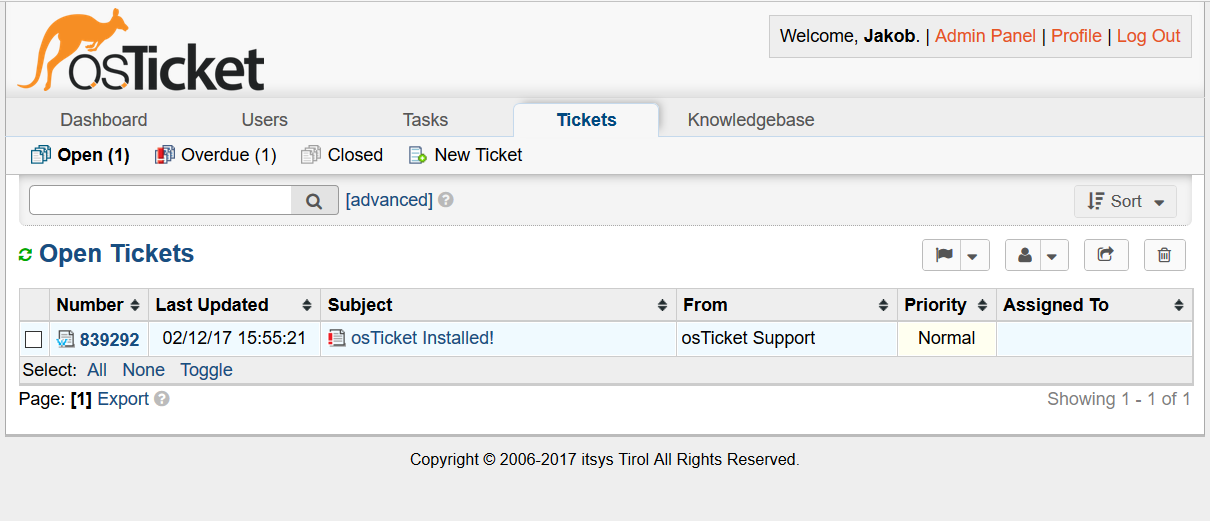
\includegraphics[scale=0.62]{figures/osticket.png}
		\caption{Die standard-Weboberfläche für Administratoren}
		\label{OSTicket Admin WebGUI}
	\end{figure}

	\subsubsection{M"oglichkeiten mit OSTicket}
	OSTicket ist sehr anpassbar. Ticketformulare und Formularfelder lassen sich mit geringem Aufwand anpassen, je nach den spezifischen Anforderungen des Helpdesks. Sollte einmal ein wahrer Sturm an Tickets eingehen, ist auch das kein Problem. Tickets lassen sich simpel priorisieren und filtern. Noch mehr Übersicht bringt die M"oglichkeit, Tickets in Hilfsthematiken einzustufen. Sollten mehrere Supportmitarbeiter gleichzeitig Arbeiten, geschieht dies ohne Problem: Ticketkollisionen werden automatisch mit Sperrvariablen vermieden.
	
	\subsubsection{Warum OSTicket?}
	Es gibt viele Gründe die für die Verwendung der Plattform OSTicket sprechen. OSTicket findet bereits bei einigen Schulen in Tirol Anwendung. Dies soll beibehalten und auf weitere Schulen ausgeweitet werden.
	\\
	Die Vorteile dieser Verbreitung und der damit einher gehenden Standardisierung kann für die Schulen große Vorteile mit sich bringen. Die bis jetzt verwendeten Systeme sind sehr unterschiedlich und in keiner Weise miteinander kompatibel. OSTicket soll als anwenderfreundliches System diese Schwierigkeiten vermeiden und beseitigen. Dadurch soll eine bessere Kommunikation zwischen Systembetreuern und IT Managern an Tirols Schulen ermöglicht werden.

	\subsection{Bootstrap}
	Das Framework Bootstrap wird verwendet, um eine Anwender freundliche Mobile-first Oberfläche zu erstellen. Bootstrap bietet umfangreiche Gestaltungsvorlagen wie Formulare, Buttons, Tabellen und weitere nützliche Oberflächengestaltungssysteme.
	
	\begin{figure}[h]
		\centering
		
\includegraphics[scale=0.65]{figures/twitter-bootstrap.jpg}
		\caption{Twitter Bootstrap Logo}
		\label{Bootstrap_Logo}
	\end{figure}
	
	Gründe die für die Verwendung von Bootstrap sprechen:
	\begin{itemize}
		\item Responsive-Design
		\item Hohe Kompatibilität bezüglich Browser
		\item Übersichtliche Dokumentation 
		\item Eine Vielzahl von Templates ist verfügbar
	\end{itemize}
\begin{figure}[h]
	\centering
	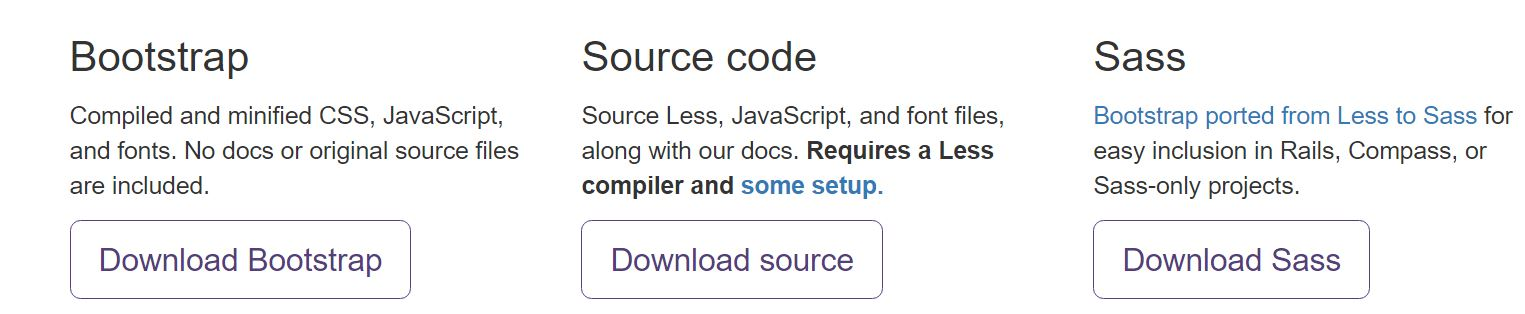
\includegraphics[scale=0.7]{figures/bootstrap.jpg}
	\caption{Bootstrap ist ein vielseitiges und anpassbares Framework}
	\label{Bootstrap Page Screenshot}
\end{figure}
	\subsection{PHP}
	OSTicket basiert auf der Skriptsprache PHP. PHP ist ein rekursives Akronym und bedeutet "Hypertext Preprocessor". PHP kann direkt in HTML\footnote{Hypertext Markup Language, definiert das Grundgerüst einer Webseite} eingebettet werden. Die Skriptsprache bietet eine Vielzahl an Funktionen Out Of The Box, wie zum Beispiel das Senden und Empfangen von Emails, Manipulation einer Datenbank oder das Befüllen einer Webseite mit Inhalten.
	
	\begin{figure}[h]
		\centering
		
\includegraphics[scale=.6]{figures/php_logo.png}
		\caption{PHP Ver. 7 Logo}
		\label{PHP_Logo}
	\end{figure}
	
	PHP ist der etablierte Standard, wenn es um serverseitige Webprogrammierung geht. Serverseitige Webprogrammierung findet statt, wenn ein Benutzer mit seinem Browser\footnote{Software zum Benutzen des World Wide Web; Bspw. Microsoft Internet Explorer, Mozilla Firefox} eine Webseite ansurft. Es wird eine sogenannte HTTP-Anfrage an den Webserver (welcher unter der Webseitenadresse erreichbar ist) gesendet. Dieser analysiert die Anfrage (welche Seite der Benutzer sehen will) und befüllt das HTML-Grundgerüst mit dynamischen Inhalten. Dann wird die Seite über das Internet zurück zum Browser des Benutzers übertragen und dargestellt.
	
	Ein großer Vorteil von PHP ist, dass es für Einsteiger in die Programmierung gut zu erlernen ist, dennoch aber äußerst flexibel, um auch umfangreiche Anwendungen (Wie OSTicket) umsetzen zu können. \\
	Die Flexibilität von PHP zeigt sich auch in der Freiheit, es auf vielen unterschiedlichen Betriebssystem wie Microsoft Windows, Apple OSX und einer Vielzahl an Linuxdistributionen verwenden zu können. Auch allerhand Webserver verstehen PHP wie ihre Muttersprache: Apache, IIS und nginx, um nur einige zu nennen.
	
	\subsection{MySQL}
	MySQL ist ein Datenbanksystem das weltweit verbreitet ist. Es gibt eine Open-Source-Sofware aber auch eine kommerzielle Enterpriseversion.
	
	\begin{figure}[h]
		\centering
		
\includegraphics[scale=.35]{figures/mysql_logo.png}
		\caption{MySQL Logo}
		\label{MySQL_Logo}
	\end{figure}
	
	MySQL wird für die Datenspeicherung von Webservices verwendet. Es wird meistens zusammen mit dem Apache Webserver und der Skiptsprache PHP verwendet. Dies war auch der Grund weshalb wir MySQL verwenden da OSTicket in der Skriptsprache PHP geschrieben ist.
	MySQL und die Bibliotheken sind hauptsächlich in C und C++ geschrieben. Dies ist zurückzuführen auf die Erzielung einer gute Performance.
	MySQL sieht grundsätzlich eine MySQL-Server vor auf dem mehrere Datenbanken erstellt werden können. In einer Datenbank könne auch mehrere Tabellen erstellt werden.
	
	\newpage
	\section{Werkzeuge}
	Die im Zuge der Projektdurchführung verwendeten Werkzeuge eignen sich für das Projekt aus verschiedenen Gründen.
	
	Ein wichtiger Punkt war die Vertrautheit mit den Werkzeugen: Ein Großteil dieser war uns bereits bekannt beziehungsweise vertraut. Des Weiteren ist die große Community im Internet sehr hilfreich bei auftretenden Problemen und Fragestellungen; meist ist die Lösung innerhalb weniger Minuten gefunden. Da es sich um weit verbreitete Entwicklungsumgebungen handelt konnte auch in der Zukunft (während der Zeit der Projektdurchführung) mit der Weiterentwicklung und Verbesserung dieser Tools gerechnet werden.
	
	\subsection{NetBeans}
	Die integrierte Entwicklungsumgebung NetBeans ist in Java geschrieben und bietet vielerlei Funktionen wie einen umfangreichen Editor, eine passable Codevervollständigung, Code Analysetools, Debugger und kann mit hilfreichen Plug-Ins wie beispielsweise EasyUML, einem Programm zum Erstellen von UML-Klassendiagrammen aus einem vorhandenen Projekt, erweitert werden. Wie in der Abbildung \ref{Netbeans_GUI} zu sehen ist, kann das Farbthema der Entwicklungsumgebung angepasst werden. Das schont die Augen und erhöht den Workflow.
	
	\begin{figure}[h]
		\centering
		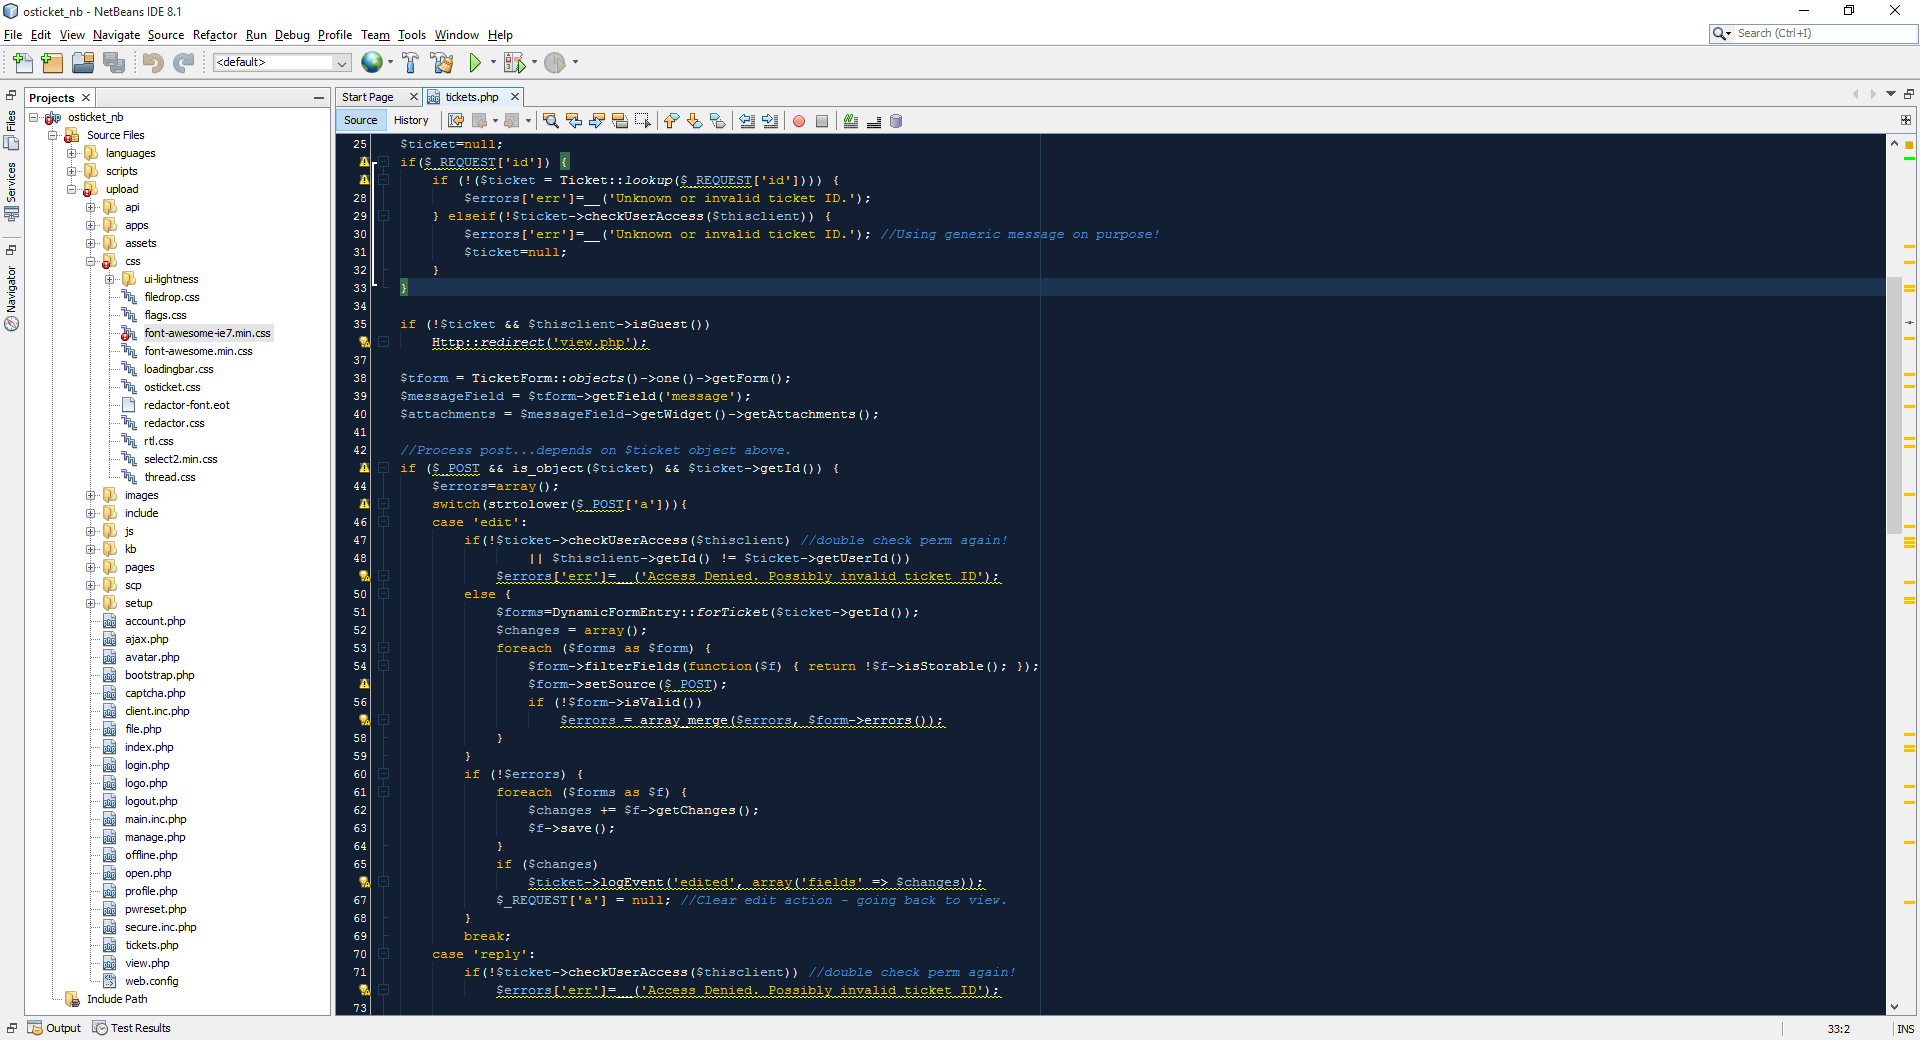
\includegraphics[scale=.3]{figures/netbeans_gui.png}
		\caption{Netbeans User Interface}
		\label{Netbeans_GUI}
	\end{figure}
	
	\begin{wrapfigure}{r}{0.4\textwidth}
		\vspace{-1cm}
		\begin{center}
			\caption{Netbeans IDE Logo}
			\vspace{.5cm}
			
\includegraphics[scale=.39]{figures/netbeans_logo.jpg}
			
			\label{Netbeans_Logo}
		\end{center}
	\end{wrapfigure}
	
	NetBeans unterstützt Programmiersprachen wie Java, PHP, C/C++ und andere. Des Weiteren ist NetBeans plattformunabhängig - wir als Projektteam haben somit die freie Wahl unter welchem Betriebssystem gearbeitet werden soll - die Kompatibilität unserer Ergebnisse ist jederzeit gegeben.
	\\
	Jedes neue Release wird auch von der Community getestet und evaluiert. Somit ist auch eine Hilfestellung bei Problemen gegeben.
	\subsection{XAMPP Apache}
	XAMPP ist eine Zusammenführung von freier Software. Es ermöglicht einfache Installation und Konfiguration des Webservers Apache und der Datenbank MariaDB. Weitere Anwendungen geliefert unter XAMPP sind die FTP-Server ProFTPd oder FileZilla Server, der Mailserver Mercury, der webbasierte Datenbankclient phpMyAdmin und andere offene Software.
	
	
	\begin{figure}[h]
		\centering
		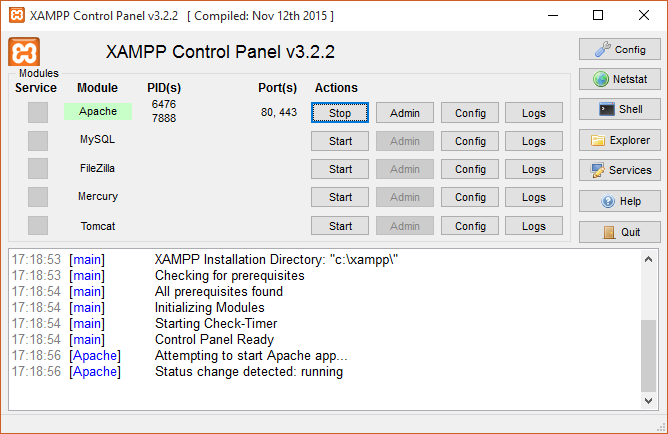
\includegraphics[scale=.8]{figures/xampp_gui.png}
		\caption{XAMPP Control Panel}
		\label{XAMPP_GUI}
	\end{figure}

	\begin{wrapfigure}{r}{0.4\textwidth}
		\vspace{-1cm}
		\begin{center}
			\caption{XAMPP Logo}
			\vspace{.5cm}
			
\includegraphics[scale=.2]{figures/xampp_logo.jpg}
			
			\label{XAMPP_Logo}
		\end{center}
	\end{wrapfigure}

	\newpage
	XAMPP ermöglicht eine einfache und schnelle Installation einer Testumgebung. Da XAMPP ausschließlich für Testumgebungen gedacht ist sind standardmäßige Sicherheitseinstellungen nicht ausreichend und ist somit nicht für Produktivumgebungen geeignet.
	
	
	\subsection{MySQL Workbench}
	Die Verwaltung der Verwendeten MySQL Datenbank erfolgt mit dem Tool MySQL Workbench. Die vielen Überwachungs- und Konfigurationsmöglichkeiten, die die GUI\footnote{Graphical User Interface} bietet, macht es möglich, auf aufwändige SQL-Skripte zu verzichten. Damit ist eine einfache Verwaltung und ein erleichterter Umgang mit dieser umfangreichen Datenbank gegeben.
	
	\begin{figure}[h]
		\centering
		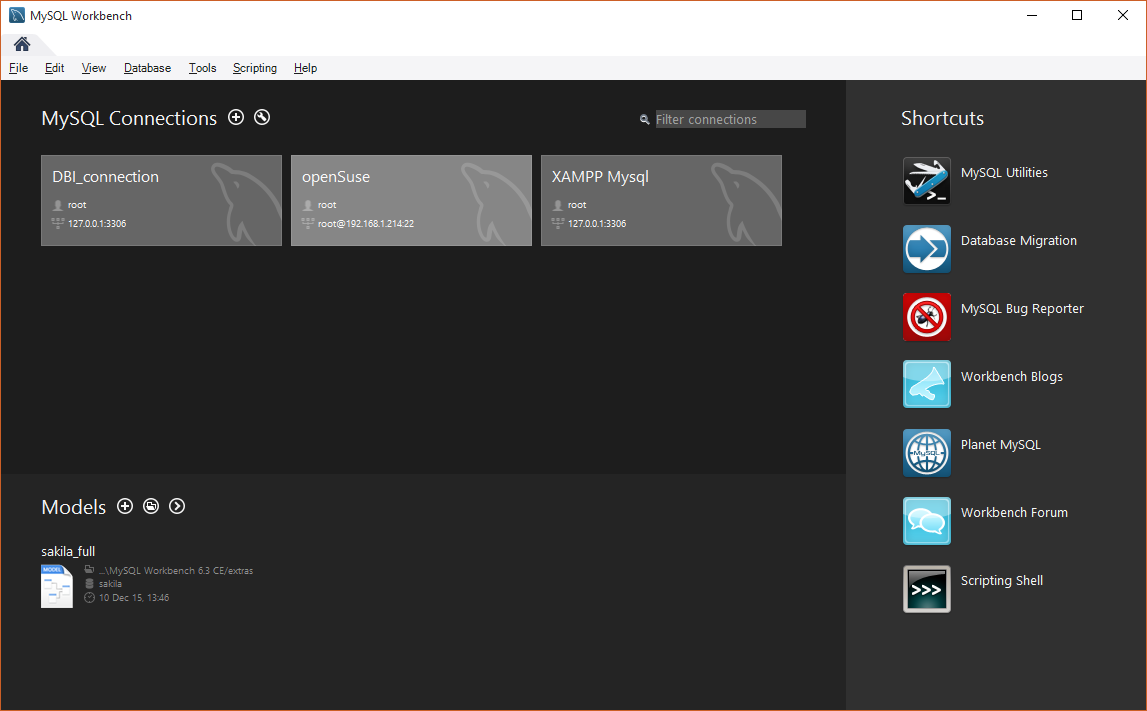
\includegraphics[scale=.5]{figures/workbench_startgui.png}
		\caption{MySQL Workbench Start Screen}
		\label{Worbench_Startgui}
	\end{figure}

	Auch die Unterstützung von Projektbetreuern und weiteren Lehrpersonen kann in Betracht gezogen werden, da die MySQL Workbench im Unterricht oft Verwendung findet.
	
	\newpage

	\begin{figure}[h]
		\centering
		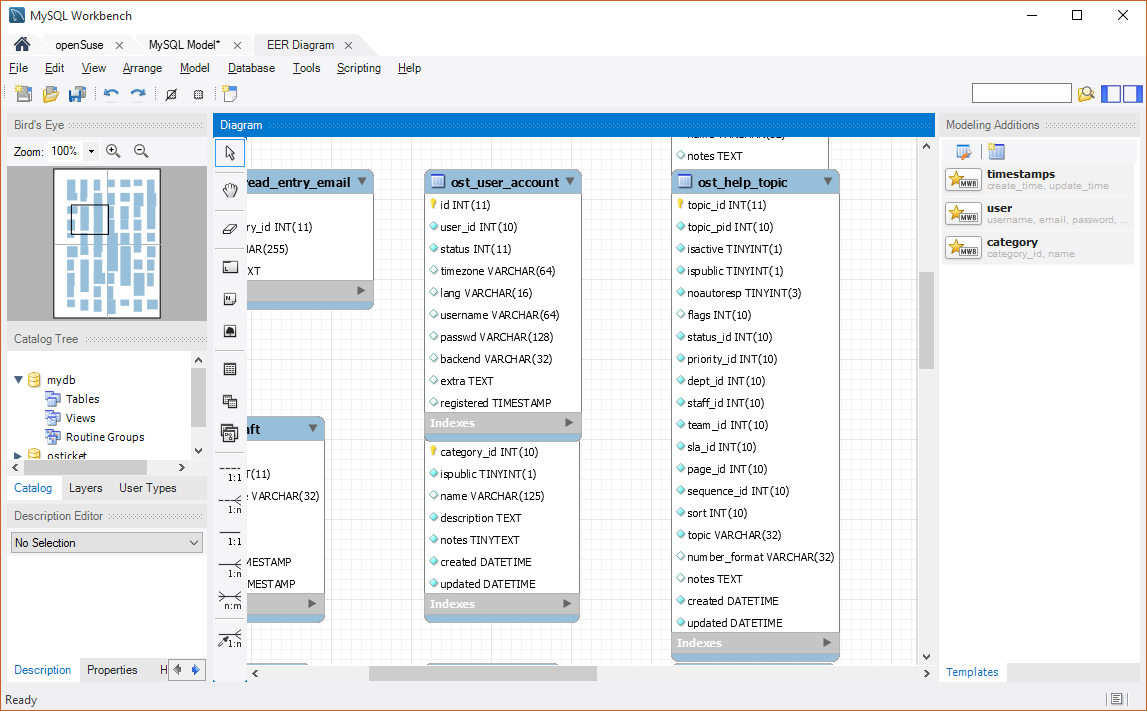
\includegraphics[scale=.5]{figures/workbench_reverse.png}
		\caption{MySQL Workbench - Datenbankdiagramm (Ausschnitt)}
		\label{Workbench_DiaGUI}
	\end{figure}
		
	MySQL Workbench kann neben der Ausführung von Konfigurations- und Datenmanipulationsbefehlen auch Modellierung: Mit dem Integrierten UML Editor kann eine Datenbank (und die zugehörigen SQL Befehle) generiert werden. Auch die entgegengesetzte Richtung ist möglich: Mit wenigen Klicks kann ein UML Diagramm aus einer bestehenden Datenbank erstellt werden. Abbldung \ref{Workbench_DiaGUI} zeigt ein solches Klassendiagramm im Detail.
	
		
	\newpage
	\section{Modelle}
	\subsection{Klassendiagramm}
	Abbildung \ref{Klassendiagramm_System} soll die Klassen welche unter dem Ticketsystem Verwendung finden umreißend beschreiben. Das Diagramm dokumentiert nicht den kompletten systematischen Aufbau des Ticketsystems in seinem "Vanilla-Zustand"\footnote{"Vanilla" beschreibt ein System oder Produkt, welches in keinster Weise verändert (customized) worden ist.}, sondern ist eine Zusammenfassung der wichtigsten Klassen, die Anwendung finden und soll lediglich veranschaulichen, welche die fundamentalsten Klassen sind und in welchem Zusammenhang diese stehen.
	\begin{figure}[h]
		\centering
		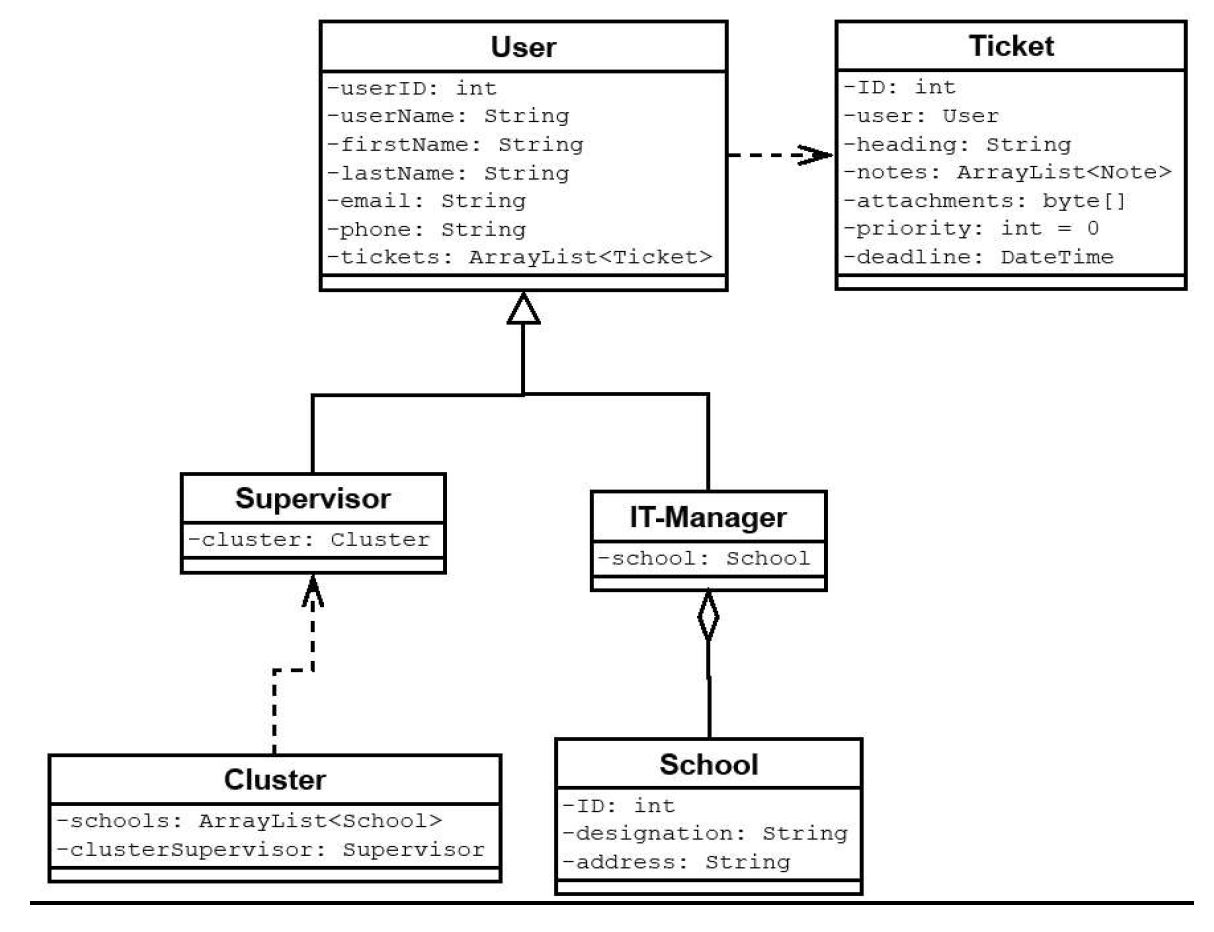
\includegraphics[scale=0.9]{figures/Klassendiagramm.jpg}
		\caption{Komprimiertes Klassendiagramm}
		\label{Klassendiagramm_System}
	\end{figure}
	\newpage
	\subsection{Komponentendiagramm}
	\begin{figure}[h]
		\centering
		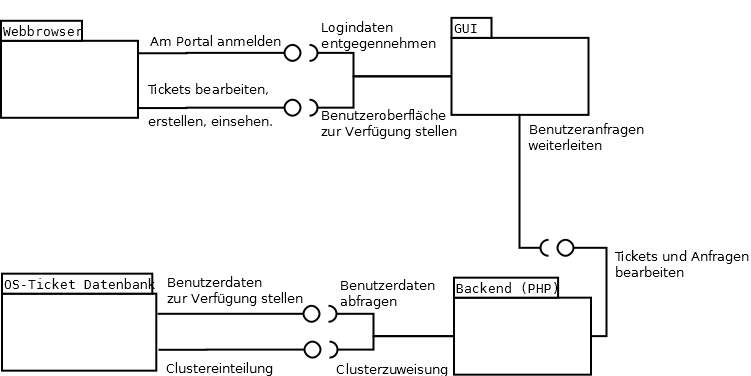
\includegraphics[scale=0.6]{figures/Komponentendiagramm.png}
		\caption{Komponentendiagramm}
		\label{Komponentendiagramm}
	\end{figure}

	\newpage
	\section{Implementierung}
	Bis jetzt wurden wichtige GUI Elemente erstellt und bezüglich der Funktionalität mit unserem Projektpartner besprochen.
	\begin{figure}[h]
		\centering
		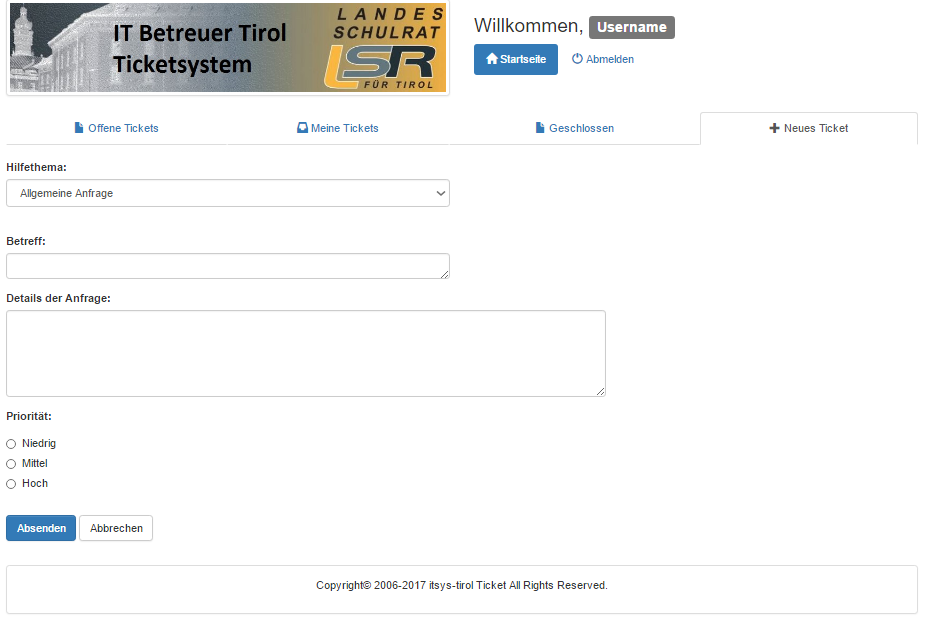
\includegraphics[scale=0.6]{figures/newTicket.png}
		\caption{Ticket erstellen}
		\label{Ein Ticket erstellen}
	\end{figure}
	\begin{figure}[h]
		\centering
		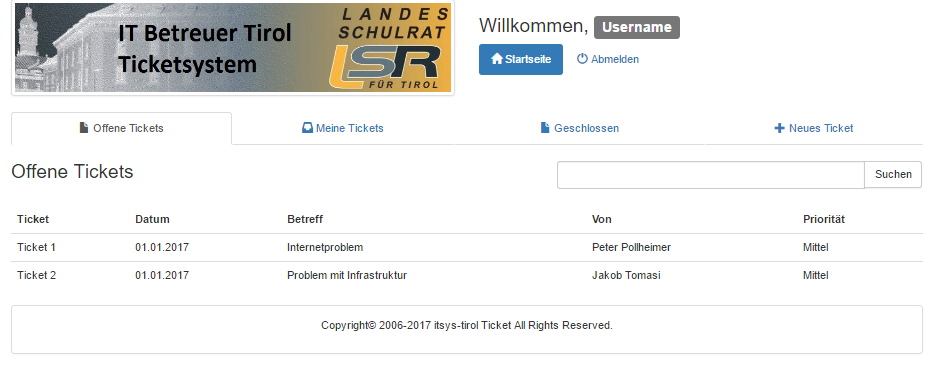
\includegraphics[scale=0.6]{figures/index.png}
		\caption{Ticketverwaltung}
		\label{Tickets verwalten}
	\end{figure}
	

%todo: Abklären, ob Position der OST-DB Doku hier angemessen ist
% Elias' OST DB DOKU:
\newpage
\section{Datenbankentwurf}
\def \currentAuthor{Elias Gabl}

\subsection{Tabellenbeschreibung der Datenbank von OSTicket}

In dieser Dokumentation finden Sie eine grobe Beschreibung der Datenbank des Systems OS Ticket. OS Ticket ist ein Ticketsingsystem das für einfache Support Anwendung Entwickelt worden ist. Die Datenbank besteht aus 59 Tabellen von diesen sind manche nicht mehr aktuell bzw. werden nicht mehr gebraucht aber sind dennoch vorhanden. Daher werden in dieser Dokumentation nur die wichtigsten Tabellen der Datenbank beschrieben.\\
Bei gewissen Spalten ist es leider nicht möglich den Inhalt anzugeben da es keine gute Dokumentation der Datenbank gibt und man den Inhalt der Spalten aus dem Kontext schließen muss.
\newline
\newline
An dieser Stelle sollte eigentlich ein Datenmodell sein aber da dieses von OSTicket recht groß und komplex ist hat es hier nicht Platz aber Sie finden es auf dem mitgelieferten Datenträger.(Der Dateiname ist: OSTicketDB.mwb).

\newpage

\subsubsection{ost\_config}

In dieser Tabelle werden wichtige Informationen über das System OSTicket gespeichert. Die Werte werden mit einem Schlüssel in die Datenbank gespeichert (Key und Value).
Diese Tabelle hat keine Referenz zu anderen Tabellen.

\begin{table}[h]
	\begin{tabular}{|p{3.5cm}|p{4cm}|p{6.2cm}|}
		\hline
		\textbf{Column Name:} & \textbf{Datatype:} & \textbf{Content:}\\
		\hline
		id & INT(11) & Eindeutg ID der Information. Dieser Wert ist rein technisch und hat  neben der Eindeutigkeit keine weitere 
		Aussagekraft. \\
		\hline
		namespace & VARCHAR(64) & \\
		\hline
		key & VARCHAR(64) & Key der Information um die Suche zu erleichtern\\
		\hline
		value & TEXT & Informations Inhalt\\
		\hline
		updated & DATETIME & Erstelldatum der Information\\
		\hline
	\end{tabular}
	\caption{tab:ost-config}
\end{table}
\label{tab:ost_config}
\newpage


\subsubsection{ost\_attachment}

Sämtliche Informationen über den Anhang eines Tickets finden sich in dieser Tabelle. Dies beinhaltet den Datentyp, Name, und id des Anhanges. 

\begin{table}[h]
	\begin{tabular}{|p{3.5cm}|p{4cm}|p{6.2cm}|}
		\hline
		\textbf{Column Name:} & \textbf{Datatype:} & \textbf{Content:} \\
		\hline
		id & INT(10) & Eindeutige ID des Anhanges. Dieser Wert ist rein technisch und hat  neben der Eindeutigkeit keine weitere  \\
		\hline
		object\_id & int(11) & Referenz auf ein Object das dem Anhang übergeben wird \\
		\hline
		type & CHAR(1) & Datentyp des Anhanges \\
		\hline
		file\_id & int(11) & Referenz auf das File das sich im Anhang befindet\\
		\hline
		name & VARCHAR(255) & Name des Anhanges \\
		\hline
		inline & TINYINT(1) & Beschreibt den Zitierstil des Anhangs \\
		\hline
		lang & VARCHAR(16) & Die Sprache in der, der Anhang verfasst wurde \\
		\hline
	\end{tabular}
	\caption{tab:ost-attachment}
\end{table}
\label{tab:ost_attachment}

\newpage

\subsubsection{ost\_canned\_response}

In dieser Tabelle werden vorgefertigte Antworten für Tickets gespeichert. Über die Antwort wird der Titel, die Sprache, der Inhalt, Erstelldatum und das Änderungsdatum gespeichert.

\begin{table}[h]
	\begin{tabular}{|p{3.5cm}|p{4cm}|p{6.2cm}|}
		\hline
		\textbf{Column Name:} & \textbf{Datatype:} & \textbf{Content:}\\
		\hline
		canned\_id & INT(10) & Eindeutige ID der Nachricht. Dieser Wert ist rein technisch und hat  neben der Eindeutigkeit keine weitere 
		Aussagekraft.\\
		\hline
		dept\_id & int(10) & Referenz auf die Abteilungen die diese Nachricht verwenden können\\
		\hline
		isenabled & TINYINT(1) & Gibt an ob die Nachricht freigegeben ist oder nicht.\\
		\hline
		titel & VARCHAR(255) & Titel der Nachricht\\
		\hline
		response & TEXT & Text den die Nachricht beinhaltet\\
		\hline
		lang & VARCHAR(16) & Sprache der Nachricht\\
		\hline
		notes & TEXT & Anmerkung zur Nachricht\\
		\hline
		created & DATETIME & Erstelldatum der Nachricht\\
		\hline
		updated & DATETIME & Änderungsdatum der Nachricht\\
		\hline
	\end{tabular}
	\caption{tab:ost-canned-response}
\end{table}
\label{tab:ost_canned_response}

\newpage

\subsubsection{ost\_content}

In dieser Tabelle werden Inhalte der Seiten gehalten. Es wird angeben ob der Inhalt aktiv ist oder nicht. Jeder Inhalt hat auch eine Titel und eine Body. Es werden auch noch der Typ und das Erstell/Änderungsdatum angegeben.

\begin{table}[h]
	\begin{tabular}{|p{3.5cm}|p{4cm}|p{6.2cm}|}
		\hline
		\textbf{Column Name:} & \textbf{Datatype:} & \textbf{Content:}\\
		\hline
		id & INT(10) & Eindeutige ID des Contents. Dieser Wert ist rein technisch und hat  neben der Eindeutigkeit keine weitere 
		Aussagekraft.\\
		\hline
		isactive & TINYINT(1) & Gib an ob der Inhalt aktiv ist oder nicht\\
		\hline
		type & VARCHAR(32) & Gib den Typ vom Inhalt an\\
		\hline
		name & VARCHAR(255) & Name vom Inhalt\\
		\hline
		body & TEXT & Der Bodyinhalt des Seiten Content\\
		\hline
		notes & TEXT & Anmerkungen zum Content\\
		\hline
		created & DATETIME & Erstelldatum des Content\\
		\hline
		updated & DATETIME & Änderungsdatum des Content\\
		\hline
	\end{tabular}
	\caption{tab:ost-content}
\end{table}
\label{tab:ost_content}

\newpage

\subsubsection{ost\_department}

Diese Tabelle speichert Informationen über eine Abteilung. Jede Abteilung hat einen Namen und eine Signatur. Ein Feld das angibt ob die Abteilung öffentlich ist oder nicht. Es wird auch festgehalten zu welcher Gruppe die Abteilung gehört und wann die Abteilung erstellt worden ist.

\begin{table}[h]
	\begin{tabular}{|p{3.5cm}|p{4cm}|p{6.2cm}|}
		\hline
		\textbf{Column Name:} & \textbf{Datatype:} & \textbf{Content:}\\
		\hline
		id & INT(10) & Eindeutige ID der Abteilung. Dieser Wert ist rein technisch und hat  neben der Eindeutigkeit keine weitere 
		Aussagekraft.\\
		\hline
		pid & INT & Referenz zu der Tabelle ost\_plugin \\
		\hline
		tpl\_id & INT(10) & Referenz zum verwendeten Template für die Abteilung\\
		\hline
		sla\_id & INT(10) & Referenz zur verwendeten Sla Vorlage\\
		\hline
		email\_id & INT(10) & Referenz zu der Verwendeten E-Mail der Abteilung\\
		\hline
		autores\_email\_id & INT(10) & \\
		\hline
		manager\_id & INT(10) & Referenz zum User der zum Manager der Abteilung ernannt wurde\\
		\hline
		flags & INT(10) & \\
		\hline
		name & VARCHAR(128) & Name der Abteilung \\
		\hline
		signature & TEXT & Signatur der Abteilung \\
		\hline
		ispublic & TINYINT(1) & Gib an ob die Abteilung öffentlich sichtbar ist \\
		\hline
		group\_membership & TINYINT(1) & Gib an zu welcher Gruppe die Abteilung gehört \\
		\hline
		ticket\_auto\_ response & TINYINT(1) & Das vordefinierte Standartticket der Abteilung \\
		\hline
		message\_auto\_ response & TINYINT(1) & Die vordefinierte Standartantwort der Abteilung auf Tickets \\
		\hline
		path & VARCHAR & Pfad der Abteilung\\
		\hline
		updated & INT(10) & Änderungsdatum der Abteilung\\
		\hline
		created & INT(10) & Erstelldatum der Abteilung\\
		\hline
	\end{tabular}
	\caption{tab:ost-department}
\end{table}
\label{tab:ost_department}

\newpage


\subsubsection{ost\_faq}

In dieser Tabelle werden die meist gestellten Fragen und die Antworten dazu gespeichert. Weiteres werden noch Schlüsselwörter und Anmerkungen zur Frage gespeichert.

\begin{table}[h]
	\begin{tabular}{|p{3.5cm}|p{4cm}|p{6.2cm}|}
		\hline
		\textbf{Column Name:} & \textbf{Datatype:} & \textbf{Content:}\\
		\hline
		faq\_id & INT(10) & Eindeutige ID der Frage. Dieser Wert ist rein technisch und hat  neben der Eindeutigkeit keine weitere 
		Aussagekraft.\\
		\hline
		category\_id & INT(10) & Referenz zu der Kategorie der die Frage zugeordnet ist  \\
		\hline
		ispublished & TINYINT(1) & Gib an ob die Frage öffentlich abrufbar ist oder nicht\\
		\hline
		question & VARCHAR(255) & Die Frage\\
		\hline
		answer & TEXT & Die Antwort zur Frage\\
		\hline
		keywords & TINYTEXT & Die Schlüsselwörter der Frage \\
		\hline
		notes & TEXT & Anmerkung zur Frage\\
		\hline
		created & DATETIME & Erstelldatum der Frage\\
		\hline
		updated & DATETIME & Änderungsdatum der Frage\\
		\hline
	\end{tabular}
	\caption{tab:ost-faq}
\end{table}
\label{tab:ost_faq}

\newpage

\subsubsection{ost\_staff}

Diese Tabelle hält sämtliche Informationen über die Staff Mitglieder des Systems OSTicket. Es wird der Vorname, Nachname, Username, das Passwort, die Email-Adresse, die Telefonnummer, die Sprache, ob das Mitglied aktiv ist, ob das Mitglied ein Administrator ist usw. gespeichert.
Die Tabelle enthält auch Informationen über die Abteilung und die Rolle des Mitglieds.


\begin{table}[h]
	\begin{tabular}{|p{3.5cm}|p{4cm}|p{6.2cm}|}
		\hline
		\textbf{Column Name:} & \textbf{Datatype:} & \textbf{Content:}\\
		\hline
		staff\_id & INT(11) & Eindeutige ID des Mitgliedes. Dieser Wert ist rein technisch und hat neben der Eindeutigkeit keine weitere 
		Aussagekraft.\\
		\hline
		dept\_id & INT(10) & Referenz zur Abteilung des Mitgliedes \\
		\hline
		role\_id & INT(10) & Referenz zur Rolle des Mitgliedes\\
		\hline
		username & VARCHAR(32) & Der Username des Mitgliedes\\
		\hline
		firstname & VARCHAR(32) & Der Vorname des Mitgliedes\\
		\hline
		lastname & VARCHAR(32) &  Der Nachname des Mitgliedes\\
		\hline
		passwd & VARCHAR(128) & Das Passwort des Mitgliedes in Hash Form \\
		\hline
		backend & VARCHAR(32) & \\
		\hline
		email & VARCHAR(128) & Die Email-Adresse des Mitgliedes \\
		\hline
		phone & VARCHAR(24) & Die Telefonnummer des Mitgliedes \\
		\hline
		phone\_ext & VARCHAR(6) & Referenz zur Email an die, die Info zum Ticketeingang geschickt wird \\
		\hline
		mobile & VARCHAR(24) & Die Handynummer des Mitgliedes \\
		\hline
		signature & TEXT & Die Signatur des Mitgliedes \\
		\hline
		lang & VARCHAR(16) & Die Sprache des Mitgliedes \\
		\hline
		timezone & VARCHAR(64) & Die Zeitzone in der sich das Mitglied befindet \\
		\hline
		locale & VARCHAR(16)& Wo sich das Mitglied genau befindet(Ort, Stadt, Land) \\
		\hline
		notes & TEXT & Anmerkungen zum Mitglied\\
		\hline
		isactive & TINYINT(1) & Gib an ob das Mitglied aktiv ist\\
		\hline
		isadmin & TINYINT(1) & Gib an ob das Mitglied ein Administrator ist\\
		\hline
			\end{tabular}
			\caption{tab:ost-staff}
		\end{table}
		\label{tab:ost_staff}
		\newpage
		\begin{table}[h]
			\begin{tabular}{|p{3.5cm}|p{4cm}|p{6.2cm}|}
		\hline
		isvisible & TINYINT(1) & Gib an ob das Mitglied für andere sichtbar ist \\
		\hline
		onvacation & TINYINT(1) & Gib an ob der Mitarbeiter im Urlaub ist \\
		\hline
		assigned\_only & TINYINT(1) & \\
		\hline
		show\_assigned\_ tickets & TINYINT(1) & Hat das Mitglied zugeteilte Tickets \\
		\hline
		changed\_passwd & TINYINT(1) & Gib an ob das Mitglied das Passwort schon mal geändert hat\\
		\hline
		max\_page\_size & INT(11) & Gibt die maximale Anzahl an Tickets an die auf der Übersichtsseite des Mitgliedes angezeigt werde \\
		\hline
		auto\_refresh\_rate & INT(10) & Gib die Taktrate an wie oft die Übersichtsseite des Mitgliedes automatisch aktualisiert werden soll \\
		\hline
		default\_signature\_ type & ENUM('none', 'mine', 'dept') & Gib die default Signatur bei der Beantwortung eines Tickets an \\
		\hline
		default\_paper\_size & ENUM('Letter', 'Legal', 'Ledger', 'A4', 'A3') & Gib das default Format der Antwort auf ein Ticket an \\
		\hline
		extra & TEXT & Hier können zusätzliche Informationen über das Mitglied gespeichert werden \\
		\hline
		permissions & TEXT & Die Zugriffsrechte des Mitgliedes \\
		\hline
		created & DATETIME & Erstelldatum des Mitgliedes \\
		\hline
		lastlogin & DATETIME & Datum an dem sich das Mitglied zuletzt angemeldet hat \\
		\hline
		passwdreset & DATETIME & Datum vom letzten rücksetzten des Passwortes \\
		\hline
		updated & DATETIME & Änderungsdatum des Mitgliedes \\
		\hline
	\end{tabular}
	\caption{tab:ost-staff2}
\end{table}
\label{tab:ost_staff2}

\newpage

\subsubsection{ost\_ticket}

Diese Tabelle enthält sämtlicher Informationen über ein Ticket. Dazu gehören der User der das Ticket abgesetzt hat, die Erkennungsnummer, die Email-Adresse des Absenders, das Thema des Tickets und wer es bearbeiten muss. Es gibt auch ein Feld das speichert ob man auf das Ticket schon geantwortet hat, wann es erstellt und gegebenenfalls verändert worden ist und ob es schon geschlossen worden ist.


\begin{table}[h]
	\begin{tabular}{|p{3.5cm}|p{4cm}|p{6.2cm}|}
		\hline
		\textbf{Column Name:} & \textbf{Datatype:} & \textbf{Content:}\\
		\hline
		ticket\_id & INT(11) & Eindeutige ID des Tickets. Dieser Wert ist rein technisch und hat  neben der Eindeutigkeit keine weitere 
		Aussagekraft.\\
		\hline
		number & VARCHAR(20) & Ticket Erkennungsnummer \\
		\hline
		user\_id & INT(11) & Referenz zum User der das Ticket abgesetzt hat.\\
		\hline
		user\_email\_id & INT(11) & Referenz zur Email-Adresse des Users der das Ticket abgesetzt hat\\
		\hline
		status\_id & INT(10) & Referenz zum Status des Tickets\\
		\hline
		dept\_id & INT(10) &  Referenz zur Abteilung der das Ticket zugewiesen wurde\\
		\hline
		sla\_id & INT(10) & Referenz zum Sla des Tickets\\
		\hline
		topic\_id & INT(10) & Referenz zum Thema dem das Ticket zugeordnet worden ist\\
		\hline
		staff\_id & INT(10) & Referenz zur Tabelle ost\_staff \\
		\hline
		team\_id & INT(10) & Referenz zum Team dem das Ticket zugewiesen worden ist \\
		\hline
		email\_id & INT(10) & Referenz zur Email an die, die Info zum Ticketeingang geschickt wird \\
		\hline
		lock\_id & INT(10) & Referenz zur Tabelle ost\_lock \\
		\hline
		flags & INT(10) &  \\
		\hline
		ip\_address & VARCHAR(64) & Die IP-Adresse von der das Ticket abgesetzt worden ist \\
		\hline
			\end{tabular}
			\caption{tab:ost-ticket}
		\end{table}
		\label{tab:ost_ticket}
		\newpage
		\begin{table}[h]
			\begin{tabular}{|p{3.5cm}|p{4cm}|p{6.2cm}|}
		\hline
		source & ENUM(Web, Email, Phone, API, Other) &\\
		\hline
		source\_extra & VARCHAR(40)&\\
		\hline
		isoverdue & TINYINT(1) & Gib an ob der Bearbeiter überfällig mit der Bearbeitung ist\\
		\hline
		isanswered & TINYINT(1) & Gib an ob dem Absender des Tickets schon geantwortet wurde\\
		\hline
		duedate & DATETIME & Gib an bis wann das Ticket bearbeitet sein sollte\\
		\hline
		est\_duedate & DATETIME & Bis wann es geplant ist das Ticket bearbeitet zu haben \\
		\hline
		reopened & DATETIME & Gib an wann ein geschlossenes Ticket zuletzt geöffnet worden ist \\
		\hline
		closed & DATETIME & Speichert das Datum an dem das Ticket geschlossen worden ist \\
		\hline
		lastupdate & DATETIME & Gib das letzte Änderungsdatum an \\
		\hline
		created & DATETIME & Erstelldatum des Tickets\\
		\hline
		updated & DATETIME & Änderungsdatum des Tickets\\
		\hline
	\end{tabular}
	\caption{tab:ost-ticket2}
\end{table}
\label{tab:ost_ticket2}

\newpage


\subsubsection{ost\_user}

Hier werden die User gespeichert die keine Mitglieder sind. Diese User können im OS Ticketsystem nur Tickets abschicken. Es wird der Name, der Status und wann er erstellt worden ist gespeichert. Weiteres kann er auch einer Organisation zugeordnet werden.

\begin{table}[h]
	\begin{tabular}{|p{3.5cm}|p{4cm}|p{6.2cm}|}
		\hline
		\textbf{Column Name:} & \textbf{Datatype:} & \textbf{Content:}\\
		\hline
		id & INT(10) & Eindeutige ID des Users. Dieser Wert ist rein technisch und hat  neben der Eindeutigkeit keine weitere 
		Aussagekraft.\\
		\hline
		org\_id & INT(10) & Referenz auf die Organisation die der User zugeordnet ist\\
		\hline
		default\_email\_id& INT(10) & \\
		\hline
		status & INT(10) & Gibt den Status des Users an\\
		\hline
		name & TEXT & Name des Users\\
		\hline
		created & DATETIME & Erstelldatum des Users\\
		\hline
		updated & DATETIME & Änderungsdatum des Users\\
		\hline
		
	\end{tabular}
	\caption{tab:ost-user}
\end{table}
\label{tab:ost_user}

\newpage

\subsubsection{ost\_user\_account}

Hier wird auf Basis der ost\_user Tabelle ein Account abgespeichert.Der Account enthält eine Referenz auf einen User. Der Account besteht aus folgenden Informationen: Status des Users, die Sprache, in welcher Zeitzone er sich aufhält, den Username, das Passwort und wann er registriert wurde.

\begin{table}[h]
	\begin{tabular}{|p{3.5cm}|p{4cm}|p{6.2cm}|}
		\hline
		\textbf{Column Name:} & \textbf{Datatype:} & \textbf{Content:}\\
		\hline
		id & INT(11) & Eindeutige ID des Accounts. Dieser Wert ist rein technisch und hat  neben der Eindeutigkeit keine weitere 
		Aussagekraft.\\
		\hline
		user\_id & INT(10) & Referenz auf den User dem der Account gehört\\
		\hline
		status& INT(11) & Den Status des Users \\
		\hline
		timezone & VARCHAR(64) & Gibt die Zeitzone an in dem sich der User befindet\\
		\hline
		lang & VARCHAR(16) & Die Sprache des Users\\
		\hline
		username & VARCHAR(64) & Username des Users\\
		\hline
		passwd & VARCHAR(128) & Das Passwort des Users in Hash form\\
		\hline
		backend & VARCHAR(32) &\\
		\hline
		extra & TEXT & Zusatz Informationen zum User\\
		\hline
		registered & TIMESTAMP & Hält fest wann sich der User registriert hat\\
		\hline
		
	\end{tabular}
	\caption{tab:ost-user-account}
\end{table}
\label{tab:ost_user_account}

\newpage

\subsubsection{ost\_ticket\_priotity}

Diese Tabelle enthält alle Informationen über die Priorität die ein Ticket haben kann.
Im gesamten kann ein Ticket eine von vier Prioritäten haben.

\begin{table}[h]
	\begin{tabular}{|p{3.5cm}|p{4cm}|p{6.2cm}|}
		\hline
		\textbf{Column Name:} & \textbf{Datatype:} & \textbf{Content:}\\
		\hline
		priority\_id & TINYINT(4) & Eindeutige ID der Priorität. Dieser Wert ist rein technisch und hat  neben der Eindeutigkeit keine weitere Aussagekraft.\\
		\hline
		priority & VARCHAR(60) & Beschreibt die Priorität\\
		\hline
		priority\_desc & VARCHAR(30) & Leg fest wie die Prioritäten geordnet werden \\
		\hline
		priority\_color & VARCHAR(7) & Leg die Farbe der Prioritäten fest\\
		\hline
		priority\_urgency & TINYINT(1) & Leg fest welche Dringlichkeit die Priorität hat \\
		\hline
		ispublic & TINYINT(1) & Gib an ob die Priorität öffentlich ist oder nicht\\
		\hline
	\end{tabular}
	\caption{tab:ost-ticket-priotity}
\end{table}
\label{tab:ost_ticket_priotity}

\newpage

\subsubsection{ost\_help\_topic}

Diese Tabelle speichert die Hilfsthemen. Es kann jedem Thema eine bestimmte Priorität zugeordnet werden. Weiters können Themen auch bestimmten Abteilungen, Teams, Administratoren oder Mitarbeiter zugeteilt werden.   

\begin{table}[h]
	\begin{tabular}{|p{3.5cm}|p{4cm}|p{6.2cm}|}
		\hline
		\textbf{Column Name:} & \textbf{Datatype:} & \textbf{Content:}\\
		\hline
		topic\_id & INT(11) & Eindeutige ID des Hilfsthemas. Dieser Wert ist rein technisch und hat  neben der Eindeutigkeit keine weitere Aussagekraft.\\
		\hline
		topic\_pid & INT(10) & Referenz zu einem Plugin für das Thema\\
		\hline
		isactive & TINYINT(1) & Leg fest ob das Thema aktiv ist oder nicht \\
		\hline
		ispublic & TINYINT(1) & leg fest ob das Thema für User zur Verfügung steht\\
		\hline
		noautoresp & TINYINT(3) & \\
		\hline
		flags & INT(10) & \\
		\hline
		status\_id & INT(10) & Referenz zu dem Status \\
		\hline
		priotity\_id & TINYINT(4) & Referenz zu einem Plugin für das Thema\\
		\hline
			\end{tabular}
			\caption{tab:ost-help-topic}
		\end{table}
		\label{tab:ost_help_topic}
		\newpage
		
		\begin{table}[h]
			\begin{tabular}{|p{3.5cm}|p{4cm}|p{6.2cm}|}
		\hline
		dept\_id & INT(10) & Referenz zu einer Abteilung die dieses Thema bearbeiten\\
		\hline
		staff\_id & INT(10) & Referenz zu einem Staff-Mitglied das diesem Thema bearbeitet\\
		\hline
		team\_id & INT(10) & Referenz zu einem Team das diesem Thema bearbeitet\\
		\hline
		sla\_id & INT(10) & Referenz zu einer SLA-Vorlage für das Thema\\
		\hline
		page\_id & INT(10) & Referenz zu der Seite des Themas\\
		\hline
		sequence\_id & INT(10) & Referenz zu der Sequenz für das Thema\\
		\hline
		sort & INT(10) & Gibt an wie das Thema gereiht werden soll\\
		\hline
		topic & VARCHAR(32) & Die Themen Beschreibung\\
		\hline
		number\_format & VARCHAR(32) & \\
		\hline
		notes & TEXT & Zusätzliche Informationen zu dem Thema\\
		\hline
		created & DATETIME & Erstelldatum des Themas\\
		\hline
		updated & DATETIME & Änderungsdatum des Themas\\
		\hline
		
	\end{tabular}
	\caption{tab:ost-help-topic2}
\end{table}
\label{tab:ost_help_topic2}

\newpage


\subsection{Beschreibung der Datenbankanbindung von OSTicket}
Die Datenbankanbindung in diesem System ist in der Klasse mysqli.php verankert. In dieser Klasse befinden sich Funktionen um eine Datenbankverbindung herzustellen, eine Query abzusetzen und die Verbindung wieder zu trennen.
Um diese Funktionen nutzen zu können muss die Klasse mysqli.php einfach, indem zu bearbeiteten Quellcode, mit einem Include Statement eingebunden werden.
Die Klasse besitzt im gesamten eine globale Variable namens \$\_\_db und 32 Funktionen. Die Variabel wird am Anfang der Klasse deklariert und nach dem Aufrufen der db\_connect Funktion hält sie eine Mysqli Objekt.
Im folgenden Abschnitt werden die wichtigsten Funktionen im Detail beschrieben.

\subsubsection{function db\_connect}
Diese Funktion stellt die Verbindung zu einer Datenbank her. Um eine Verbindung herstellen zu können benötigt sie folgende Parameter:
	\begin{itemize}
		\item \textbf{\$host} ist die Hostadresse unter der die Datenbank erreicht werden kann.
		\item \textbf{\$user} ist ein User der die benötigen Rechte hat um lesend und schreiben auf die Datenbank zugreifen zu können.
		\item \textbf{\$passwd} ist das Passwort des User.
		\item \textbf{\$options} ist ein Array das Informationen über den Secure Sockets Layer (SSL) und den Namen der zu selektierenden Datenbank beinhaltet
	\end{itemize}
Diese Funktion kann man als Herzstück dieser Klasse bezeichnen, da man immer zuerst eine Verbindung zu der Datenbank herstellen muss um mit ihr arbeiten zu können. Um eine andere Funktion dieser Klasse nützten zu können muss man zuerst die Funktion db\_connect aufrufen.
Eine Verbindung besteht solange bis man mit der Funktion db\_close die Verbindung beendet.
Tritt in dieser Funktion ein Fehler auf so gibt sie den Wert null zurück.
\newpage

\begin{lstlisting}[language=PHP, caption=mysqli.php/function-db\_connect1, firstnumber=21]
function db_connect($host, $user, $passwd, $options = array()) {
global $__db;

//Assert
if(!strlen($user) || !strlen($host))
return NULL;

if (!($__db = mysqli_init()))
return NULL;
\end{lstlisting}

In diesem Abschnitt des Codes wird zuerst die Variabel \textbf{\$\_\_db} als globale Variable deklariert. Anschließen wird durch die String-Funktion strlen geprüft welche Länge die Parameter \textbf{\$user} und \textbf{\$host} haben. Hat einer der beiden Parameter eine Länge von 0 dann liefert die Funktion den Wert null zurück.\\
Nach dem Überprüfen der beiden Parameter \textbf{\$user} und \textbf{\$host} wird bei der nächsten IF-Anweisung geprüft ob ein Mysqli Objekt instantiiert werden kann. Ist das nicht der Fall gib die Funktion wieder den Wert null zurück

\newpage

\begin{lstlisting}[language=PHP, caption=mysqli.php/function-db\_connect2, firstnumber=32]
if (isset($options['ssl']))
$__db->ssl_set(
$options['ssl']['key'],
$options['ssl']['cert'],
$options['ssl']['ca'],
null, null);
elseif(!$passwd)
return NULL;
\end{lstlisting}
In diesem Codeteil wird zuerst überprüft ob im Array \$options Werte mit dem Schlüssel 'ssl' abgelegt sind wenn das der Fall ist übergibt er die Werte 'key', 'cert', und 'ca' der Datenbankverbindung. Nach der Überprüfung des Arrays überprüft er noch ob ein Passwort gesetzt ist, ist keines gesetzt gibt die Funktion wieder null zurück.

\newpage

\begin{lstlisting}[language=PHP, caption=mysqli.php/function-db\_connect3, firstnumber=41]
$port = ini_get("mysqli.default_port");
$socket = ini_get("mysqli.default_socket");
$persistent = stripos($host, 'p:') === 0;
if ($persistent)
$host = substr($host, 2);
if (strpos($host, ':') !== false) {
list($host, $portspec) = explode(':', $host);
// PHP may not honor the port number 
// if connecting to 'localhost'
if ($portspec && is_numeric($portspec)) {
if (!strcasecmp($host, 'localhost'))
// XXX: Looks like PHP gethostbyname() is IPv4 only
$host = gethostbyname($host);
$port = (int) $portspec;
}
elseif ($portspec) {
$socket = $portspec;
}
}

if ($persistent)
$host = 'p:' . $host;
\end{lstlisting}

In diesem Teilbereich des Codes werden Port, Socket und Hostname der Verbindung festgelegt. Zu beginn des Abschnittes wird mit Hilfe der Funktion ini\_get der default Wert vom MySql Port und Socket den Variablen \$port und \$socket zugewiesen.\\
Anschließend wird mit Hilfe der Funktion stripos der Variable \$persistent der Wert true zugewiesen wenn der Value 'p:' am Anfang des Strings \$host steht oder false wenn 'p:' nicht am Anfang des Strings zu finden ist.\\
Danach wird durch eine IF-Anweisung geprüft welchen Wert die Variable \$persistent angenommen hat. Hat sie den Wert true wird der Variable \$host durch die Funktion substr der gleiche Wert wie sie schon hatte nur ohne den ersten zwei Zeichen zugewiesen.\\
In der nächsten IF-Anweisung wird geprüft ob sich im String der Variable \$host ein ':' befindet. Befindet sich im String ein Doppelpunkt so wird alles was sich Links vom Doppelpunkt befindet der Variable \$host zugewiesen und alles was sich Recht davon befindet wird der Variable \$portspec zugewiesen. Anschließen wird geprüft ob die Variable \$portspec einen Wert hat und ob dieser Wert Nummerisch ist. Trifft beides zu wird noch geprüft ob die Variable \$host den Wert 'localhost' hat. Hat die Variable \$host nicht den Wert 'localhost' wird durch die Funktion gethostbyname die IPv4 Adresse oder der unveränderte Hostnamen der Variable \$host zugewiesen und der Variable \$port wird der zu verwendende Port zugewiesen.

\begin{lstlisting}[language=PHP, caption=mysqli.php/function-db\_connect4, firstnumber=63]
	    // Connect
	    $start = microtime(true);
	    if (!@$__db->real_connect($host, $user, $passwd, null, $port, $socket))
	    return NULL;
	    //Select the database, if any.
	    if(isset($options['db'])) $__db->select_db($options['db']);
	    
	    @$__db->query('SET NAMES "utf8"');
	    @$__db->query('SET CHARACTER SET "utf8"');
	    @$__db->query('SET COLLATION_CONNECTION=utf8_general_ci');
	    $__db->set_charset('utf8');
\end{lstlisting}
In diesem Abschnitt wird anhand der oben gesammelten Informationen die Verbindung zur Datenbank aufgebaut und die ausgewählte Datenbank selektiert.\\
Anschließend werden noch Informationen über den verwendeten Zeichencode übergeben.\\
\\
Der Rückgabewerte dieser Funktion ist, wenn keine Fehler vorkommt, eine Mysqli Objekt. 
\newpage

\subsubsection{function db\_query}

Mithilfe dieser Funktion kann man eine Query an die Datenbank schicken. Ist die Query ein SELECT Statement bekommt man ein Result Set zurück ist es aber eine Query mit einem INSERT, UPDATE oder DELETE Statement bekommt man true zurück wenn es erfolgreich war und false wenn es nicht erfolgreich war. Um eine Query absetzten zu könne benötigt diese Funktion folgende Parameter:
\begin{itemize}
	\item \textbf{\$query} Mit diesem Parameter wird die abzuschickende Query angeben.
	\item \textbf{\$logError} Dieser Parameter ist Standard mäßig immer true.
	\item \textbf{\$buffered} Dieser Parameter ist Standard mäßig immer true.
\end{itemize}

\begin{lstlisting}[language=PHP, caption=mysqli.php/function-db\_query1, firstnumber=154]
function db_query($query, $logError=true, $buffered=true) {
global $ost, $__db;

if ($__db->unbuffered_result) {
$__db->unbuffered_result->free();
$__db->unbuffered_result = false;
}
\end{lstlisting}

In diesem Teilabschnitt werden zuerst mal die Variablen \$ost und \$\_\_db als global Variablen deklariert.
Anschließen wird geprüft ob die Variable \$\_\_db ein Unbuffered Result beinhaltet. Ist dies der Fall wird das Unbuffered Result geleert und der Wert auf false gesetzt.

\newpage
\begin{lstlisting}[language=PHP, caption=mysqli.php/function-db\_query2, firstnumber=163]
$tries = 3;
do {
$res = $__db->query($query,
$buffered ? MYSQLI_STORE_RESULT : MYSQLI_USE_RESULT);
// Retry the query due to deadlock error (#1213)
// TODO: Consider retry on #1205 (lock wait timeout exceeded)
// TODO: Log warning
} while (!$res && --$tries && $__db->errno == 1213);
\end{lstlisting}

Dieser Teil des Codes schickt mit Hilfe der query Funktion eine Anfrage mit der Query an die Datenbank und speichert das Ergebnis in der Variable \$res. Anschließen wird geprüft ob die Abfrage erfolgreich war, ob \$\_\_db->errno gleich 1213 ist und zusätzlich wird die Variable \$tries um eins verkleinert. Treffen alle Argumente zu war die Query erfolglos und wird noch mal geschickt. Nach drei Versuche bricht die do-while-Schleife ab und es wird nicht mehr Versucht eine Anfrage an die Datenbank zu schicken.
War das Abschicken der Query erfolgreich wird die do-while-Schleife ebenfalls abgebrochen und die nächste IF-Anweisung wird nicht durchgeführt.  
\newpage

\begin{lstlisting}[language=PHP, caption=mysqli.php/function-db\_query3, firstnumber=173]
if(!$res && $logError && $ost) { //error reporting
// Allow $logError() callback to determine if logging is necessary
if (is_callable($logError) && !($logError($__db->errno)))
return $res;

$msg='['.$query.']'."\n\n".db_error();
$ost->logDBError('DB Error #'.db_errno(), $msg);
//echo $msg; #uncomment during debuging or dev.
}

if (is_object($res) && !$buffered)
$__db->unbuffered_result = $res;

return $res;
\end{lstlisting}

Wenn, wie im oberen Abschnitt schon erwähnt, die do-while-Schliefe den Versuch eine Query an die Datenbank zu schicken Abgebrochen hat wird als nächstes geprüft ob die Variable \$res etwas beinhaltet und ob die Variablen \$logError und \$ost deklariert wurden. Treffen alle Parameter zu wird bei der nächsten IF-Anweisung geprüft ob die Variable \$logError eine Wert beinhaltet der als Funktion aufgerufen werden kann und ob der Aufruf dieser Funktion mit dem Parameter \$\_\_db->errno false zurück gibt.
Triff dies auch zu wird die Variable \$res mit dem Wert null zurück gegeben. Anschließen wird der Variable \$msg noch der Fehlertext übergeben und es wird mit der Variable \$ost  die Funktion logDBError aufgerufen. Als Parameter werden dieser Funktion der Errorcode und der Errortext mitgegeben.
In der letzten IF-Anweisung wird noch geprüft ob die Variabel \$res ein Objekt ist und ob die Variable \$buffered den Wert false hält. Ist dies der Fall wird der Wert der Variable \$res dem Datenfeld unbuffered\_result des Objektes \$\_\_db übergeben. 
Zuletzt wird noch die Variable \$res zurückgegeben.
\newpage

\subsection{Tabellenbeschreibung der Datenbank von unserem Java EE Prototyp}
Dieser Teil der Dokumentation beschreibt die Datenbank von unserem Java EE Prototypen. Dieser Java EE Prototyp erfüllt im Grunde alle Anforderungen die an das Ticketsystem gestellt wurden.\\
Hinter dieser Anwendung steht die hier beschriebene Datenbank. Diese Datenbank wurde so konzipiert das sie einfach und Übersichtlicht ist. Es wurde auch darauf geachtet das keine unnötigen Tabellen verwendet werden müssen da wir anhand dieser Anwendung zeigen möchten wie viel unnötigen Funktionen das OSticketsystem vorweist.
Hier haben Sie ein EER-Diagramm der Datenbank für die grobe Übersicht.
\begin{figure}[h]
	\centering
	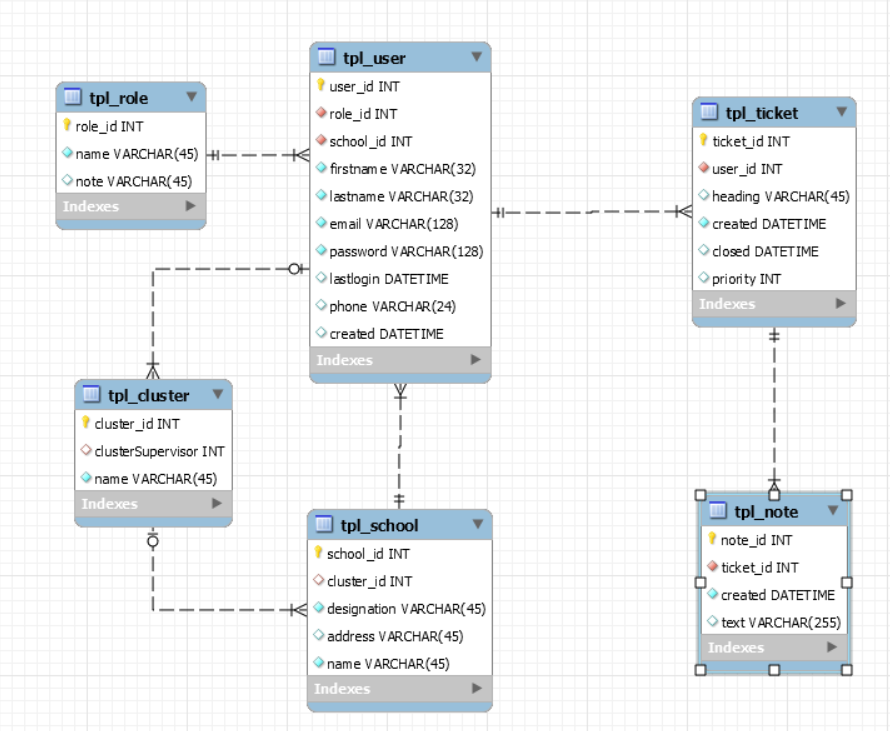
\includegraphics[scale=.8]{figures/EER-Diagramm-Java-EE-Anwendung.PNG}
	\caption{EER-Diagramm-Java-EE-Anwendung}
	\label{EER-Diagramm-Java-EE-Anwendung}
\end{figure}

\newpage

\subsubsection{tpl\_user}

In dieser Tabelle werden die User des Ticketsystems gehalten. Von einem User wird der Vorname, Nachname, E-Mail-Adresse und das Password gespeichert. Optional kann auch der letzte Login, die Telefonnummer und das Datum an dem er erstellt worden ist gespeichert werden.
Ein User muss einer Schule zugewiesen sein um vollständig im System registriert zu sein. Ein User kann auch ein Supervisor eines Clusters sein aber das ist optional.
WICHTIG: lastlogin und created werden nach folgender Form in der Datenbank gespeichert "YYYY-MM-DD HH:MM:SS".

\begin{table}[h]
	\begin{tabular}{|p{3.5cm}|p{4cm}|p{6.2cm}|}
		\hline
		\textbf{Column Name:} & \textbf{Datatype:} & \textbf{Content:}\\
		\hline
		user\_id & INT & Eindeutige ID des User. Dieser Wert ist rein technisch und hat  neben der Eindeutigkeit keine weitere Aussagekraft.\\
		\hline
		role\_id & INT( & Referenz zu der Rolle die der User besitzt\\
		\hline
		school\_id & INT &  Referenz zu der Schule vom User \\
		\hline
		firstname & VARCHAR(32) & Vorname des Users\\
		\hline
		lastname & VARCHAR(32) & Nachname des Users\\
		\hline
		email & VARCHAR(128) & E-Mail-Adresse des Users\\
		\hline
		password & VARCHAR(128) & Das Passwort des Users in Hash Form \\
		\hline
		lastlogin & DATETIME & Das Datum, in oben angegebener Form, an dem sich der User zuletzt angemeldet hat \\
		\hline
		password & VARCHAR(24) & Das Passwort des Users in Hash Form \\
		\hline
		created & DATETIME & Das Datum, in oben angegebener Form, an dem der User angelegt worden ist\\
		\hline
	\end{tabular}
	\caption{tab:tpl-user}
\end{table}
\label{tab:tpl_user}

\newpage

\subsubsection{tpl\_ticket}

In dieser Tabelle werden die erstellten Ticket des Ticketsystems gespeichert. Das Ticket wird genau einem User zugeordnet und kann mehrere Notizen(notes) haben. Des weiteren besteht ein Ticket aus einem Header, die Priorität und wann es erstellt und geschlossen worden ist.
WICHTIG: closed und created werden nach folgender Form in der Datenbank gespeichert "YYYY-MM-DD HH:MM:SS".

\begin{table}[h]
	\begin{tabular}{|p{3.5cm}|p{4cm}|p{6.2cm}|}
		\hline
		\textbf{Column Name:} & \textbf{Datatype:} & \textbf{Content:}\\
		\hline
		ticket\_id & INT & Eindeutige ID des Tickets. Dieser Wert ist rein technisch und hat neben der Eindeutigkeit keine weitere Aussagekraft.\\
		\hline
		user\_id & INT & Referenz zum User zu dem das Ticket gehört\\
		\hline
		heading & VARCHAR(45) &  Die Überschrift des Tickets\\
		\hline
		created & DATETIME & Das Datum, in oben angegebener Form, an dem das Ticket angelegt worden ist\\
		\hline
		closed & DATETIME & Das Datum, in oben angegebener Form, an dem das Ticket geschlossen worden ist\\
		\hline
		priority & INT & Hier wird die Priorität des Tickets angegeben. Kann eine Wert von 0-4 haben, der default Wert ist 0.\\
		\hline
	\end{tabular}
	\caption{tab:tpl-ticket}
\end{table}
\label{tab:tpl_ticket}

\newpage

\subsubsection{tpl\_note}

In dieser Tabelle werden die Notizen(notes) für die Tickets gespeichert. Jeder Notiz wird ein Ticket zugewiesen. Ein Ticket kann auch mehrere Notizen haben aber eine Notiz gehört immer genau zu einem Ticket. Eine Notiz besteht aus einem Text und einem Datum das angibt wann die Notiz erzeugt worden ist.
WICHTIG: created wird nach folgender Form in der Datenbank gespeichert "YYYY-MM-DD HH:MM:SS".

\begin{table}[h]
	\begin{tabular}{|p{3.5cm}|p{4cm}|p{6.2cm}|}
		\hline
		\textbf{Column Name:} & \textbf{Datatype:} & \textbf{Content:}\\
		\hline
		note\_id & INT & Eindeutige ID der Notiz. Dieser Wert ist rein technisch und hat neben der Eindeutigkeit keine weitere Aussagekraft.\\
		\hline
		ticket\_id & INT & Referenz zum Ticket dem diese Notiz angehört\\
		\hline
		created & DATETIME & Das Datum, in oben angegebener Form, an dem die Notiz angelegt worden ist\\
		\hline
		text & VARCHAR(255) & Ein Text der Informationen zum Ticket beinhaltet\\
		\hline
	\end{tabular}
	\caption{tab:tpl-note}
\end{table}
\label{tab:tpl_note}

\newpage

\subsubsection{tpl\_role}

In dieser Tabelle werden die Rollen gespeichert die ein User annehmen kann. Eine Rolle besteht lediglich aus einem Namen und einer Notiz. Ein User kann genau eine Rolle haben aber eine Rolle kann von mehreren User genutzt werden. 

\begin{table}[h]
	\begin{tabular}{|p{3.5cm}|p{4cm}|p{6.2cm}|}
		\hline
		\textbf{Column Name:} & \textbf{Datatype:} & \textbf{Content:}\\
		\hline
		role\_id & INT & Eindeutige ID der Rolle. Dieser Wert ist rein technisch und hat neben der Eindeutigkeit keine weitere Aussagekraft.\\
		\hline
		name & VARCHAR(45) & Name der Rolle\\
		\hline
		note & VARCHAR(45) & Informationen über die Rolle\\
		\hline
	\end{tabular}
	\caption{tab:tpl-role}
\end{table}
\label{tab:tpl_role}


\subsubsection{tpl\_school}

In dieser Tabelle werden die Schulen gespeichert die bei diesem Ticketsystem dabei sind.
Eine Schule wird mit Ihrer Bezeichnung, Adresse und Namen abgespeichert. Weiteres kann eine Schule einem Cluster zugeordnet werden. 

\begin{table}[h]
	\begin{tabular}{|p{3.5cm}|p{4cm}|p{6.2cm}|}
		\hline
		\textbf{Column Name:} & \textbf{Datatype:} & \textbf{Content:}\\
		\hline
		school\_id & INT & Eindeutige ID der Schule. Dieser Wert ist rein technisch und hat neben der Eindeutigkeit keine weitere Aussagekraft.\\
		\hline
		cluster\_id & INT & Referenz zu dem Cluster dem die Schule angehört\\
		\hline
		designation & VARCHAR(45) & Schulbezeichnung der Schule\\
		\hline
		address & VARCHAR(45) & Die Adresse der Schule\\
		\hline
		name & VARCHAR(45) & Name der Schule\\
		\hline
	\end{tabular}
	\caption{tab:tpl-school}
\end{table}
\label{tab:tpl_school}

\newpage

\subsubsection{tpl\_cluster}

In dieser Tabelle werden die Cluster festgelegt. Ein Cluster ist ein Mengen von Schule die zu einer Organisation zusammen geschlossen worden sind. Jeder Cluster hat einen Supervisor der für die Bearbeitung der anfallenden Ticket in diesem Cluster verantwortlich ist.
Der Supervisor wird per Referenz zur User-Tabelle festgelegt ein Cluster hat immer genau einen Supervisor. Zusätzlich wird noch ein Name für den Cluster festgelegt.

\begin{table}[h]
	\begin{tabular}{|p{3.5cm}|p{4cm}|p{6.2cm}|}
		\hline
		\textbf{Column Name:} & \textbf{Datatype:} & \textbf{Content:}\\
		\hline
		cluster\_id & INT & Eindeutige ID des Clusters. Dieser Wert ist rein technisch und hat neben der Eindeutigkeit keine weitere Aussagekraft.\\
		\hline
		clusterSupervisor & INT & Referenz zu dem User der in diesem Cluster der Supervisor ist\\
		\hline
		name & VARCHAR(45) & Name des Clusters\\
		\hline
	\end{tabular}
	\caption{tab:tpl-cluster}
\end{table}
\label{tab:tpl_cluster}

\newpage

\subsection{Beschreibung der Datenbankanbindung von unserem Java EE Prototyp}

Da unsere Anwendung nur ein Prototyp ist wurde auch die Datenbankanbindung nur mit den wichtigsten Funktionen konzipiert. Deshalb ist die Klasse Datenbankanbindung.java auch sehr statisch und redundant geschrieben. 
Die Datenbankanbindung wurde mit Hilfe der Java Api JDBC realisiert.\\
Mithilfe der get-Methoden kann man die einzelnen Tabellen aus der Datenbank auslesen und mit Hilfe der insert-Methoden kann man Einträge in die Tabellen einfügen.
Mit der Methode dbconnect stellt man die Verbindung zu der Datenbank her.\\
\\
Am Anfang der Klasse werden drei String Variablen mit Informationen über den Datenbank Zugang initialisiert.
\begin{itemize}
	\item \textbf{url} Die URl unter der die Datenbank zu erreichen ist. In diesem Fall liegt die Datenbank Local auf einem Rechner da es noch ein Prototyp ist.
	\item \textbf{username} ist ein User der die benötigen Rechte hat um lesend und schreiben auf die Datenbank zugreifen zu können. In unserem Fall greifen wir mit dem root User auf die Datenbank zu da sie ja nur Local gespeichert ist und wir uns noch keine Gedanken über Sicherheit machen müssen.
	\item \textbf{\$password} ist das Passwort des User. 
\end{itemize}
\begin{lstlisting}[language=JAVA, caption=Datenbankanbindung.java/Datenfelder, firstnumber=30]
private String url = "jdbc:mysql://localhost:3306/java_ee_database";
private String username = "root";
private String password = "";
\end{lstlisting}
\newpage
Im folgenden werden die Methoden Klasse Datenbankanbindung.java im Detail beschrieben.
 
\subsubsection{Methode dbconnect\(\)}
Diese Methode stellt eine Verbindung zu der Datenbank her und liefert ein Statement Objekt zurück. Das Statement Objekt wird benötigt um eine Query an die Datenbank zu schicken.
Um ein Statement Objekt erzeugen zu könne muss man zuerst ein Connection Objekt erzeugen. Dies erfolgt durch die Methode getConnection mit den Parameter url, username, password. Konnte keine Verbindung zu der Datenbank hergestellt werden wird durch den Catch-Block die SQLException gefangen und der Wert null zurück gegeben.

\begin{lstlisting}[language=JAVA, caption=Datenbankanbindung.java/Methode-dbconnect, firstnumber=44]
public Statement dbconnect()
{   
try
{
Connection connection = (Connection) DriverManager.getConnection(url, username, password);
Statement stmt = connection.createStatement();
return stmt;
}
catch(SQLException e)
{
return null;
}
}
\end{lstlisting}

\newpage

\subsubsection{Methode insertRole\(\)}

In dieser Methode wird ein Insert-Statement erzeugt und anschließen an die Datenbank geschickt, zurück bekommen wir den String 'Das Insert hat funktioniert.' oder null wenn das Insert nicht funktioniert hat. Als Parameter werden die Values benötigt die man in die Datenbank schreiben möchte. Zuerst wird mit der Methode dbconnect\(\) ein Statment Objekt erstellt und anschließen wird mit Hilfe der executeUpdate Methode die Query an die Datenbank geschickt. Ist das abschicken der Query nicht erfolgreich bekommt man den Wert null zurück.\\
Dieser Methodenaufbau finden wir bei allen insert-Methoden in dieser Klasse.

\begin{lstlisting}[language=JAVA, caption=Datenbankanbindung.java/Methode-dbconnect, firstnumber=271]
public String insertRole(String name, String note)
{
try
{
dbconnect().executeUpdate("INSERT INTO tpl_role 
(name, note) VALUES (\""+ name +"\", \""+ note +"\")");
return "Das Insert hat funktioniert";
}
catch(SQLException e)
{
return null;
}
}
\end{lstlisting}
\newpage
\subsubsection{Methode getRoles\(\)}

Mit der Methode getRoles kann man alle Rollen aus der Datenbanktabelle role auslesen.
Zuerst wird in dieser Methode eine ArrayList roles Initialisiert, anschließen werden String Variablen definiert die benötigt werden um aus dem ResultSet die Datenfelder der Role zu lesen.
Im try-Block wird nun ein SELECT-Statement an die Datenbank geschickt und ein ResultSet Objekt rs erzeugt. 
Um aus dem ResultSet die einzelnen Rollen auszulesen benötigen wir eine while-Schleife. Diese iterieren solange durch das ResultSet bis kein Eintrag mehr vorhanden ist(bis rs.next() false zurück gib).
In dieser while-Schleife wird zuerst ein role Objekt erzeugt und mit Hilfe der set-Methoden die Datenfelder des Rollen Objekt gesetzt. Zum Schluss wird das Rollen Objekt noch der ArrayList roles hinzugefügt. Wurde durch alle Einträge des ResultSet iteriert wird das Statement geschlossen. Tritt werden dem durchlaufen des Try-Blockes ein Fehler auf so wird durch den Catch-Block der Wert null zurückgegeben.\\ 
Dieser Methodenaufbau findet wir bei allen get-Methoden in dieser Klasse.

\newpage


\begin{lstlisting}[language=JAVA, caption=Datenbankanbindung.java/Methode-getRoles, firstnumber=59]
public ArrayList getRoles()
{
ArrayList <tpl_role> roles = new ArrayList<>();

String value = "role_id";
String value1 = "name";
String value2 = "note";
try 
{
ResultSet rs = dbconnect().executeQuery("SELECT * FROM tpl_role");

while(rs.next())
{
tpl_role role = new tpl_role();
role.setName(rs.getString(value1));
role.setId(rs.getInt(value));
role.setNote(rs.getString(value2));
roles.add(role);
}
rs.close();
return roles;
} 
catch (SQLException ex) 
{
return null;
}
}
\end{lstlisting}

\newpage


%todo: Datenbank Doku Gendern
%todo: Formatieren der Tabellen
%todo: Verschieben nach Kap. 2 (Vorstellung des Produktes; hier die JavaeEE Doku)
%todo: Dokumentation kontrollieren



%-------------------------------------
%todo: Formatierungschaos im Chapter Problemanalyse beheben und Inhalt überarbeiten
%-------------------------------------

\chapter{Problemanalyse}

\section{USE-Case-Analyse}
{\linespread{.5}
	\textbf{Akteure:}
	\begin{itemize}
		\item Systembetreuer
		\item Anwender (IT-Manager und eventuell Lehrer, in Folgendem Anwender genannt)
\end{itemize}}

\vspace{-.5cm}
\begin{table}[h]
	\centering
	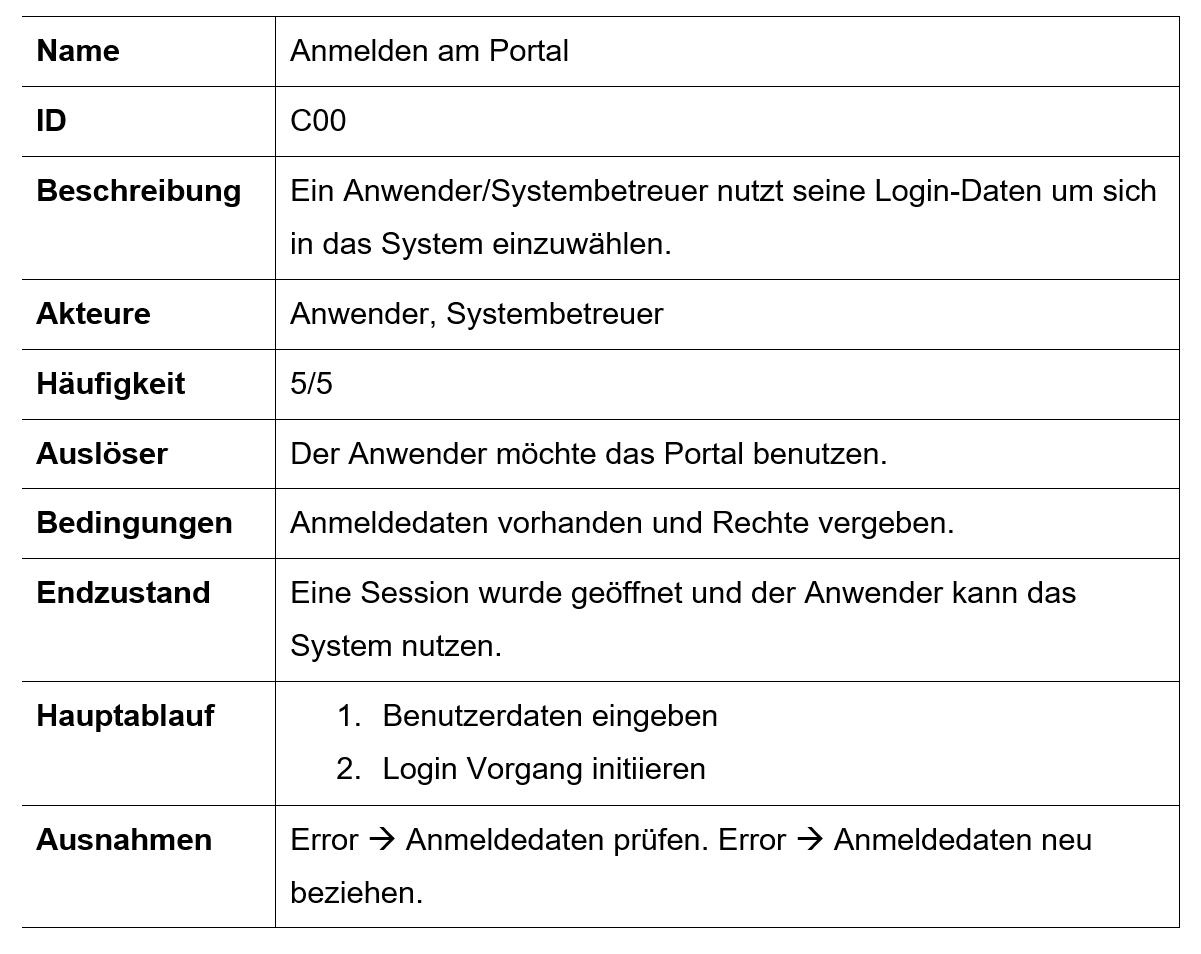
\includegraphics[scale=0.51]{figures/C00.png}
	\caption{Use-Case C00}
	\label{Abb_C00}
\end{table}
\newpage
\vspace{-.5cm}	
\begin{table}[h]
	\centering
	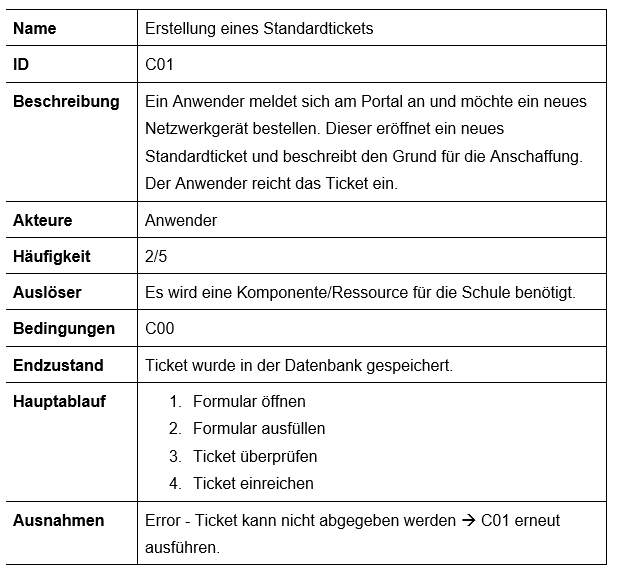
\includegraphics[scale=0.55]{figures/C01.png}
	\caption{Use-Case C01}
	\label{Abb_C01}
\end{table}
\newpage
\vspace{-.5cm}	
\begin{table}[h]
	\centering
	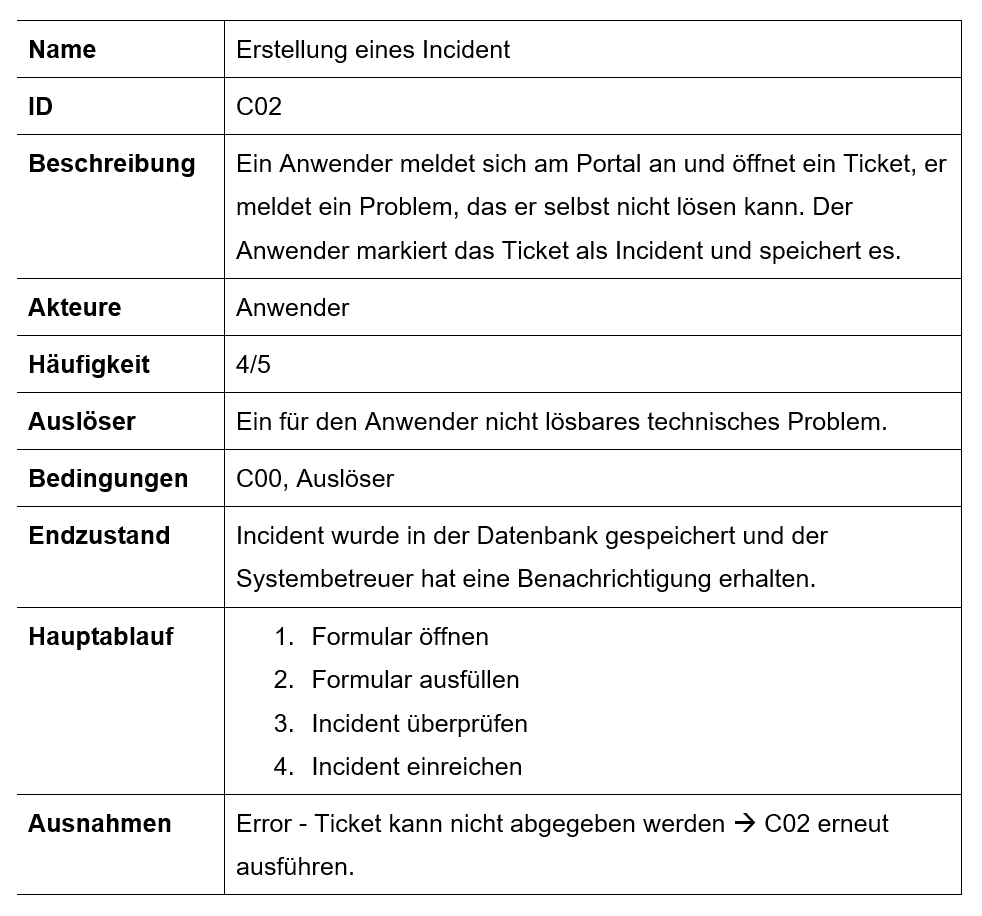
\includegraphics[scale=0.6]{figures/C02.png}
	\caption{Use-Case C02}
	\label{Abb_C02}
\end{table}

\vspace{-.5cm}	
\begin{table}[h]
	\centering
	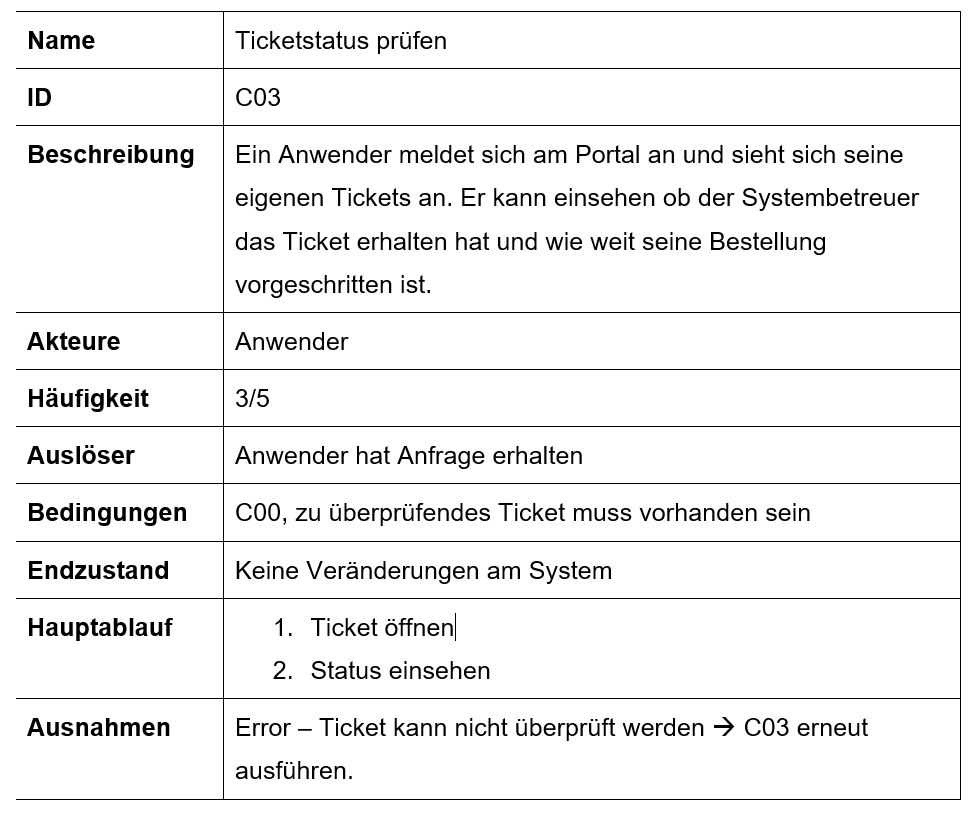
\includegraphics[scale=0.62]{figures/C03.png}
	\caption{Use-Case C03}
	\label{Abb_C03}
\end{table}
\newpage
\vspace{-.5cm}	
\begin{table}[h]
	\centering
	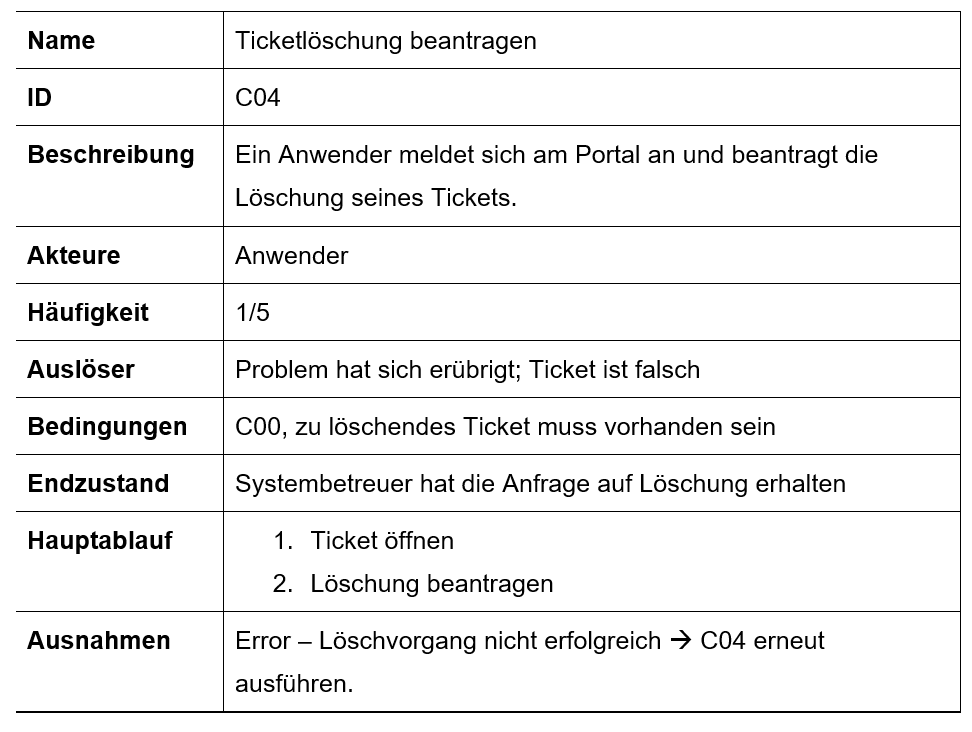
\includegraphics[scale=0.62]{figures/C04.png}
	\caption{Use-Case C04}
	\label{Abb_C04}
\end{table}


\vspace{-.5cm}	
\begin{table}[h]
	\centering
	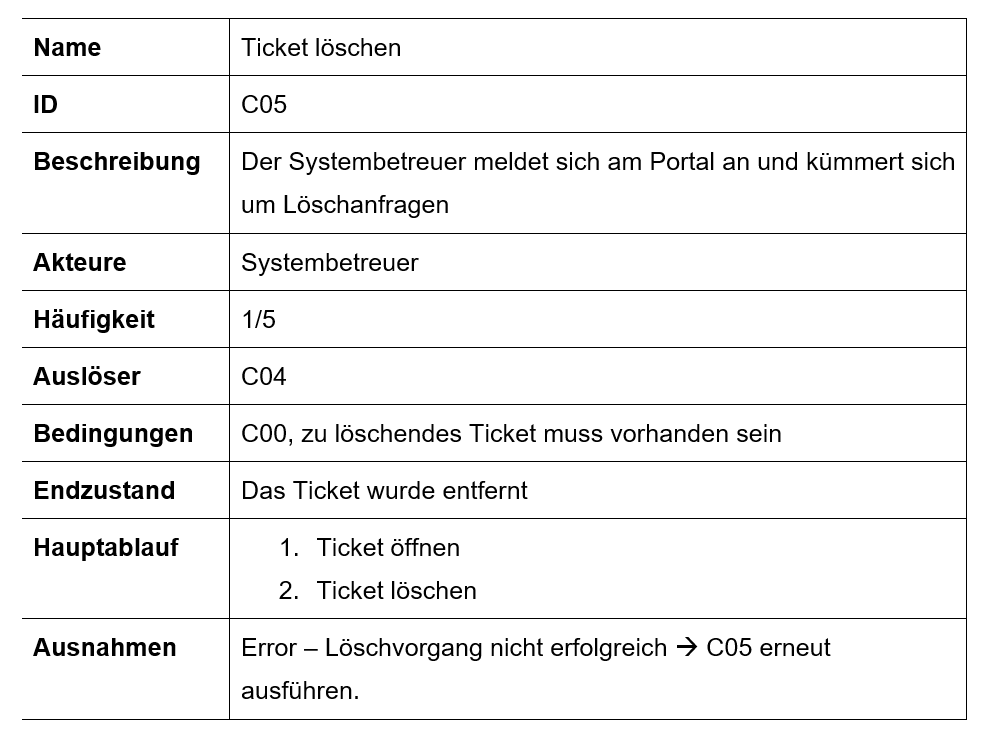
\includegraphics[scale=0.62]{figures/C05.png}
	\caption{Use-Case C05}
	\label{Abb_C05}
\end{table}
\newpage
\vspace{-.5cm}	
\begin{table}[h]
	\centering
	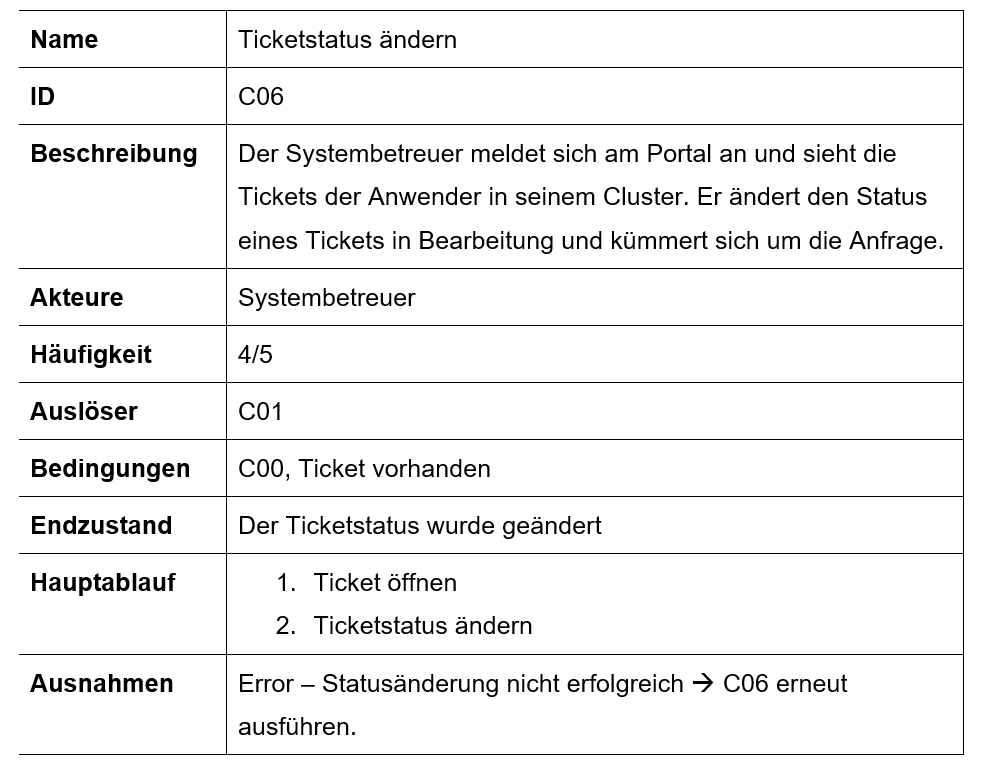
\includegraphics[scale=0.62]{figures/C06.png}
	\caption{Use-Case C06}
	\label{Abb_C06}
\end{table}
\newpage
\vspace{-.5cm}	
\begin{table}[h]
	\centering
	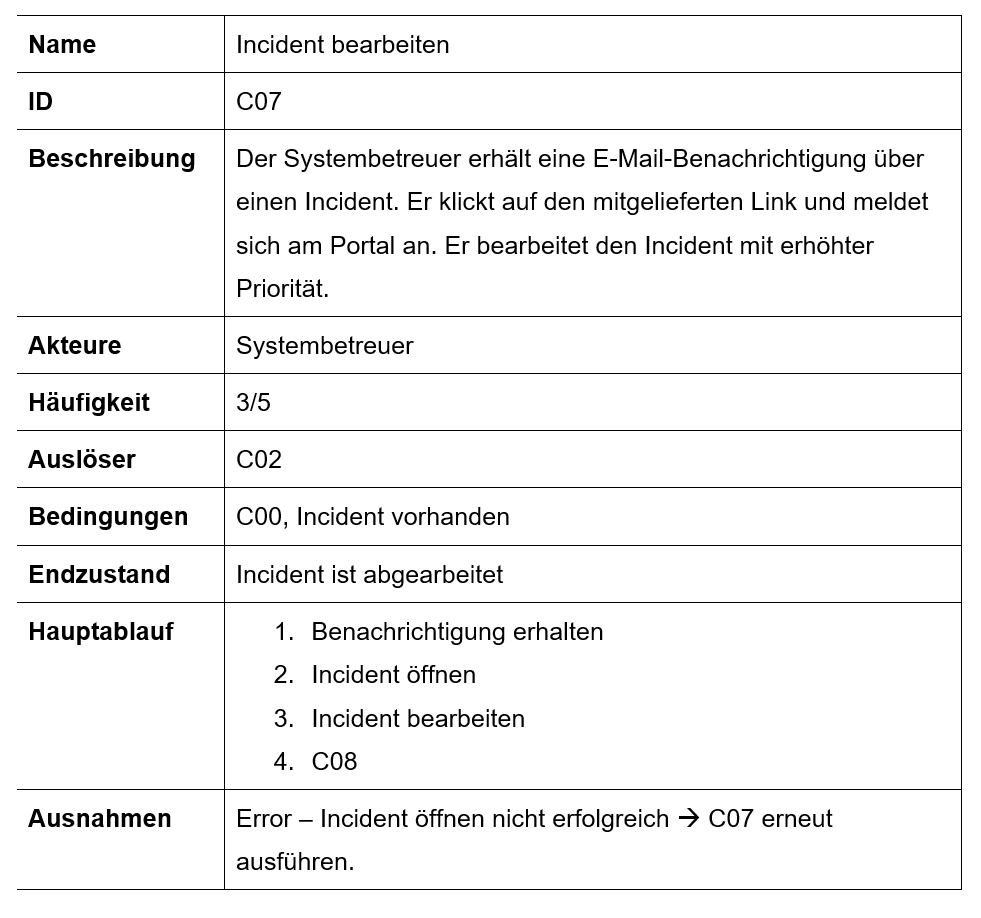
\includegraphics[scale=0.62]{figures/C07.png}
	\caption{Use-Case C07}
	\label{Abb_C07}
\end{table}

\vspace{-.5cm}	
\begin{table}[h]
	\centering
	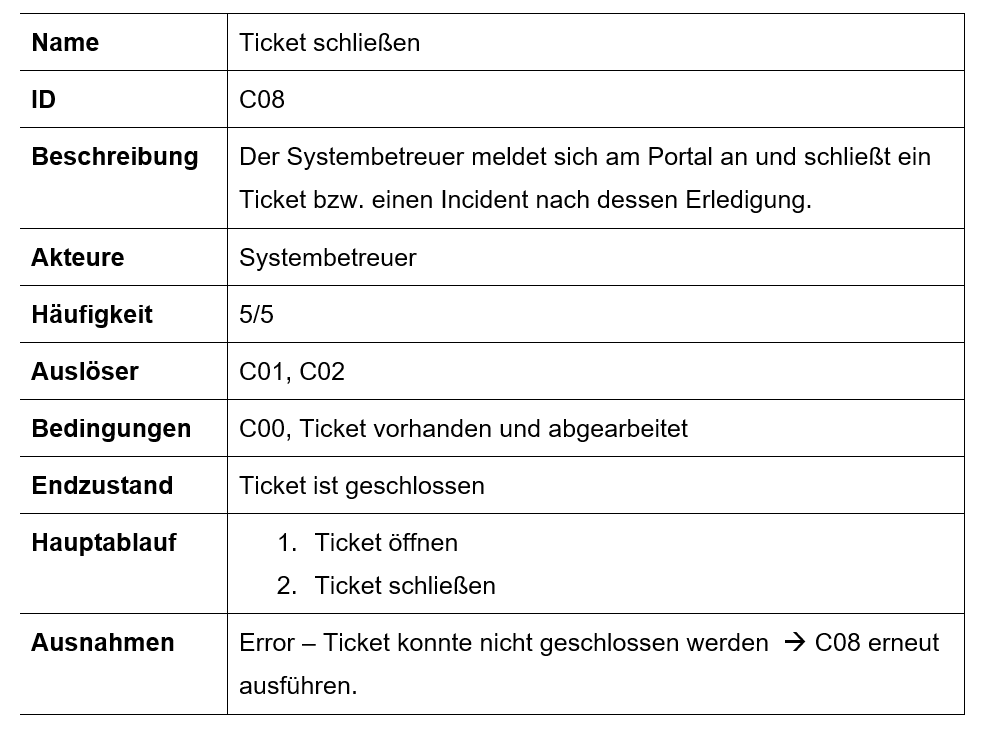
\includegraphics[scale=0.62]{figures/C08.png}
	\caption{Use-Case C08}
	\label{Abb_C08}
\end{table}


\subsection{Ablaufbeschreibung}
\textbf{C00:}
\\ 
Der Benutzer wird aufgefordert seine Benutzerdaten einzugeben.
Hat er die Daten richtig eingegeben wird er angemeldet. Sind die Daten falsch kommt er zurück zur Dateneingabe.
\\
\textbf{C01:}
\\
Der Benutzer muss zuerst ein Formular öffnen, um ein Ticket erstellen zu können. Anschließend muss das Formular ausgefüllt werden. 
\\
Nach dem Überprüfen des Tickets kann der Benutzer sich entscheiden ob er das Ticket abschickt oder ob er Änderungen vornehmen möchte. 
\\
Wenn das Abschicken fehlgeschlagen ist kommt er zum Anfang zurück. Wenn das abschicken erfolgreich war, wird das Ticket in der Datenbank gespeichert.
\\
\textbf{C02:}
\\
Der Benutzer muss zuerst ein Formular öffnen um einen Incident erstellen zu können. Anschließend muss das Formular ausgefüllt werden. Nach dem Überprüfen des Incident kann der Benutzer sich entscheiden, ob er den Incident abschickt oder ob er Änderungen vornehmen möchte.
\\
Wenn das Abschicken fehlgeschlagen ist kommt er zum Anfang zurück. Wenn das abschicken erfolgreich war wird der Incident in der Datenbank gespeichert und der Systembetreuer erhält eine Benachrichtigung.
\\
\textbf{C03:}
\\
Der Benutzer muss das Formular öffnen um den Status zu sehen. Ist das Öffnen fehlgeschlagen kommt er wieder zum Ausgangspunkt und kann es nochmal versuchen.
\\
\textbf{C04:}
\\
Um die Löschung beantragen zu können muss der Benutzer zuerst das Ticket öffnen. Danach kann er die Löschung beantragen. Schlägt dies fehl kommt er wieder zurück an den Anfang und kann es nochmal versuchen. War der Antrag auf Löschung erfolgreich erhält der Systembetreuer eine Anfrage zur Löschung.
\\
\textbf{C05:}
\\
Um ein Ticket zu löschen muss der Systembetreuer das Ticket öffnen und löschen. Schlug dies fehl kommt er wieder zurück an den Anfang und kann es nochmal versuchen. War das Löschen erfolgreich wurde das Ticket aus der Datenbank entfernt.
\\
\textbf{C06:}
\\
Um den Ticketstatus ändern zu können muss der Systembetreuer das Ticket öffnen und ändern. Schlug dies fehl kommt er wieder zurück an den Anfang und kann es nochmal versuchen. War das ändern erfolgreich wurde der Ticketstatus geändert.
\newpage
\textbf{C07:}
\\
Um ein Ticket schließen zu können muss der Systembetreuer das Ticket öffnen um es dann zu schließen. Schlug dies fehl kommt er wieder zurück an den Anfang und kann es nochmal versuchen. War das schließen erfolgreich ist das Ticket geschlossen.

\newpage
\section{Wireframes}	
\begin{figure}[h]
	\centering
	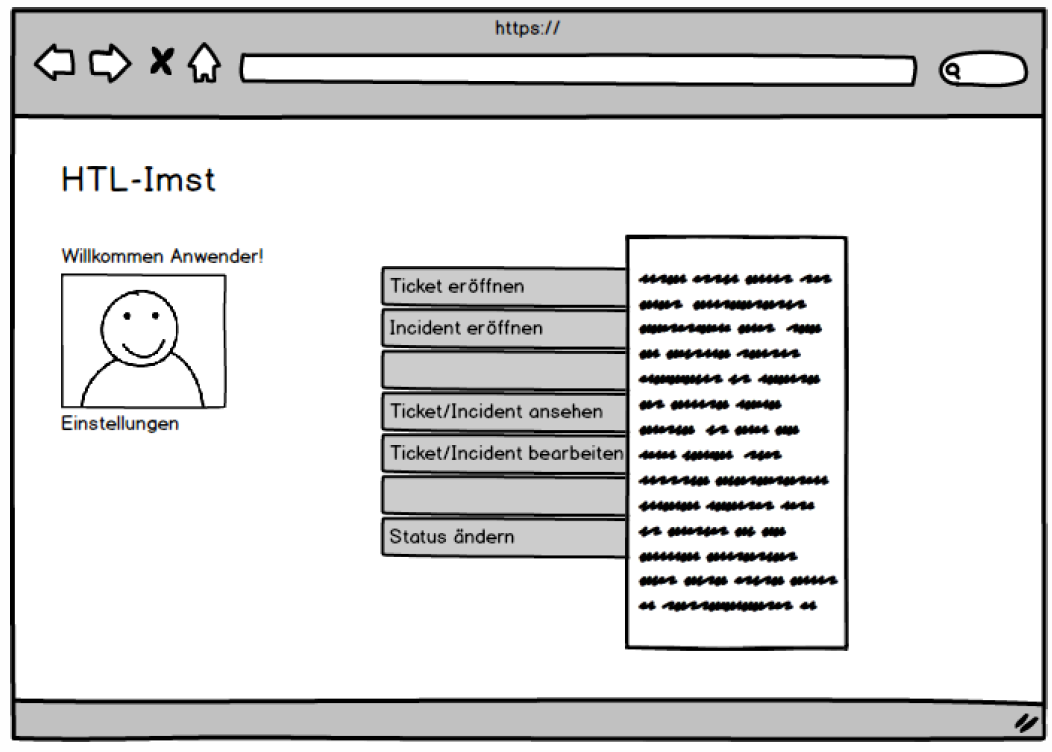
\includegraphics[scale=0.44]{figures/Wireframe_Anwender.png}
	\caption{Mockup Anwendersicht}
	\label{Abb_Mockup_Anwendersicht}
\end{figure}

\vspace{-.5cm}
\begin{figure}[h]
	\centering
	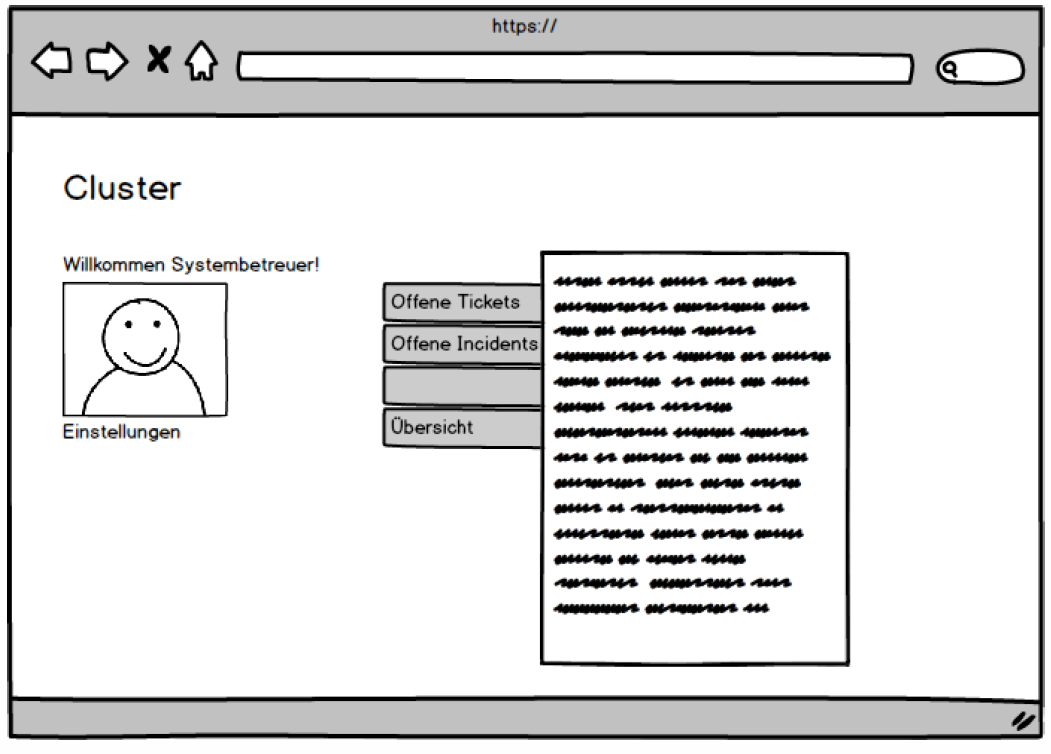
\includegraphics[scale=0.399]{figures/Wireframe_Systembetreuer.png}
	\caption{Mockup Systembetreuer}
	\label{Abb_Mockup_Systembetreuer}
\end{figure}



\vspace{.5cm}
\begin{figure}[h]
	\centering
	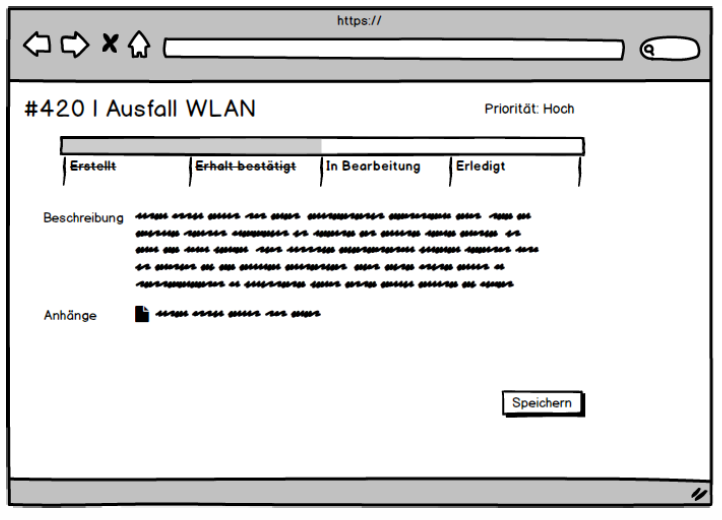
\includegraphics[scale=0.582]{figures/Wireframe_Ticket.png}
	\caption{Mockup Ticketstatus}
	\label{Abb_Mockup_Ticketstatus}
\end{figure}	

\newpage
\section{Prototyp}
\begin{figure}[h]
	\centering
	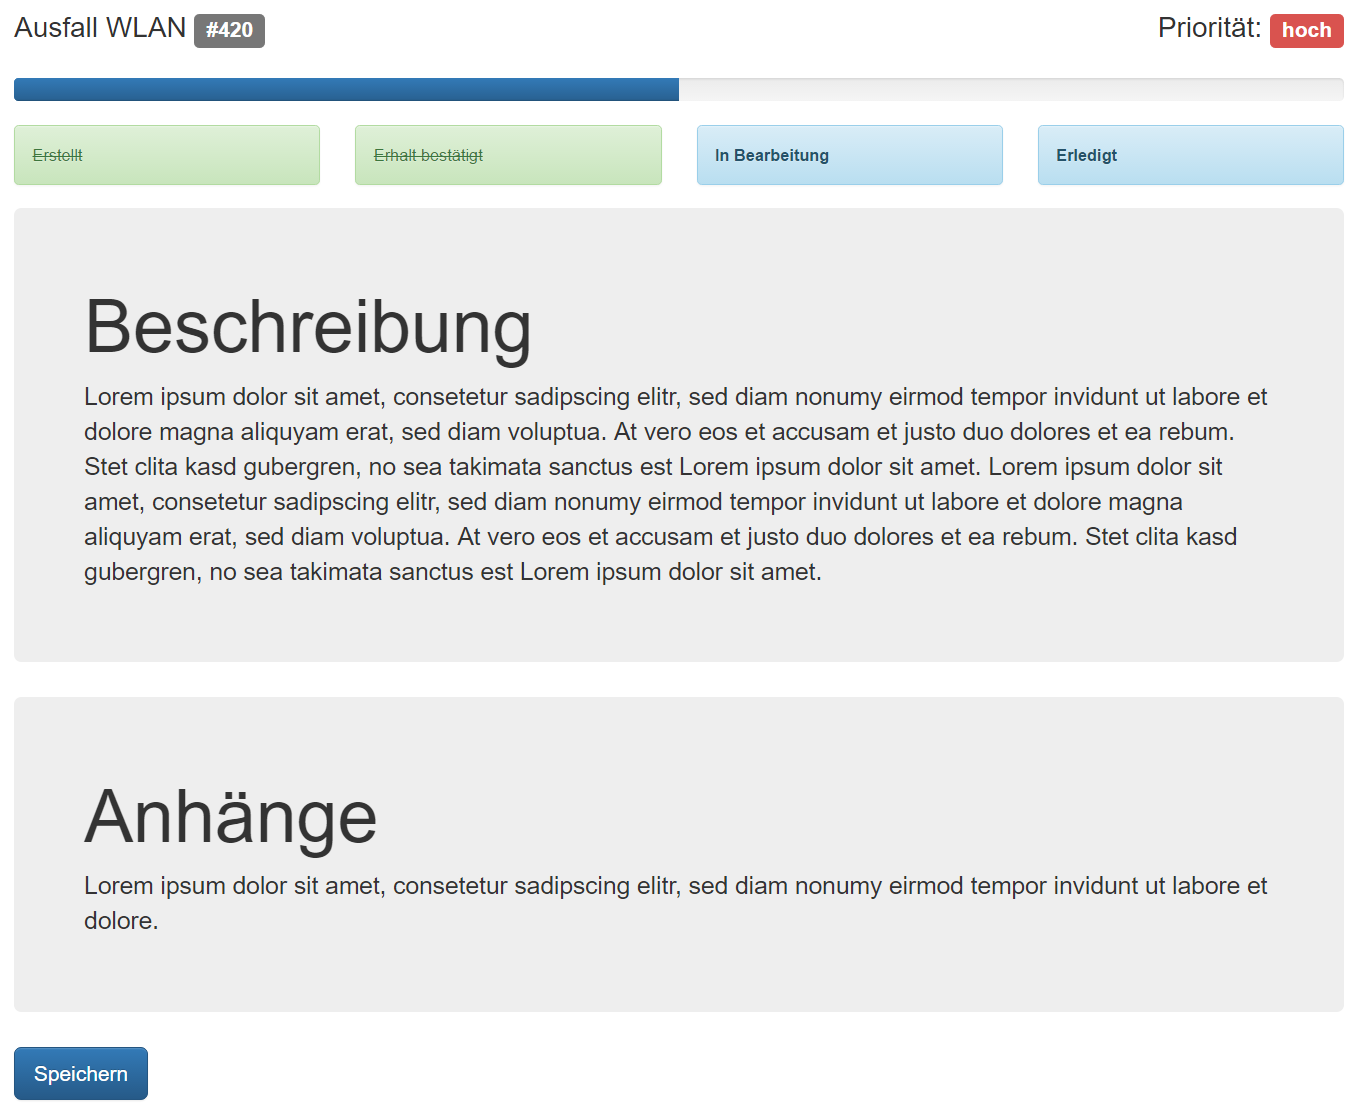
\includegraphics[scale=0.8]{figures/Prototyp.png}
	\caption{Prototyp Ticketstatus}
	\label{Abb_Prototyp_Ticketstatus}
\end{figure}


%-------------------------------------------------
%Chapter Problemanalyse Formatierungschaos bis zu diesem Punkt
%-------------------------------------------------




\newpage
\section{Domain-Class-Modelling}
\begin{itemize}
	\item "Dinge" (Rollen, Einheiten, Geräte, Events etc.) identifizieren, um die es im Projekt geht
	\item ER-Modellierung oder Klassendiagramme
	\item Zustandsdiagramme (zur Darstellung des Lebenszyklus von Domain-Klassen darstellen)
\end{itemize}

\newpage
\section{User-Interface-Design}
\begin{itemize}
	\item Mockups
	\item Wireframes
\end{itemize}



%  INPUT SYSTEMENTWURF JAVAEE (Jakob)
\chapter{Java Enterprise Prototyp}
\label{jee_proto}
\def \currentAuthor{Jakob Tomasi}
Aufgrund der bereits geschilderten Nicht-Durchführbarkeit einer Adaption von \getOst\ wurde ein Prototyp für ein Ticketsystem entworfen, welcher die vom Landesschulrat und den Tiroler Schulen benötigten Funktionen mitbringt. Die Anforderungen für dieses System sind im Grunde die gleichen, welche zu Beginn an die \getOst-Adaption gestellt wurden.
\paragraph{}
Ein Auszug dieser Anforderungen sind:

\begin{itemize}
	\item Usability: Das System soll ohne lange Schulungsphasen oder Einlernzeit verwendet werden können. Unter Verwendung ist hauptsächlich das Absetzten von Supporttickets definiert.
	\item Mobility: Das Web-Frontend soll auch auf Smartphones und Tablets verwendet werden können und die gleichen Funktionen wie auf dem PC liefern.
	\item Adaptability: Sollten sich Anforderungen, Best Practices oder Sicherheitsanforderungen ändern, sollen diese mit so geringem Aufwand als möglich implementiert werden können.
\end{itemize}

Dieser Prototyp wurde mit der Absicht erstellt, die Durchführbarkeit bzw. Machbarkeit eines Ticketsystems entsprechend den Anforderungen des Landesschulrates und insbesondere Herrn \getHammerl\ zu entsprechen. Damit wird also geklärt, dass Java Enterprise Edition als Basistechnologie für ein solches System eingesetzt werden kann. Damit besteht eine Grundlage, an der kommende Projekte anknüpfen können.

\section{Technologie}
Für den Prototyp des Ticketsystems wurde Java Enterprise Edition ausgesucht. Diese Entscheidung basiert auf der Absicht, die bei \getOst\ gezogenen Schlüsse zu beachten und die Probleme die bei \getOst\ auftraten zu vermeiden.
\paragraph{}
JavaEE erscheint hierfür besonders geeignet, da es (in dem Verwendungsmodus, der an der Schule gelehrt wurde) von sich aus das MVC-Entwurfsmuster anwendet (mehr im nächsten Abschnitt).
\paragraph{}
Des Weiteren eignet sich JavaEE für die Beseitigung der Schwächen \getOst s durch die relativ strengen Sprachkonventionen und die (beinahe) unausweichliche Objektorientierung.

\section{Architektur}
Als Basis für die Systemarchitektur wird das Model View Controller Muster verwendet. Das bedeutet die Trennung zwischen JavaBeans (Model), die direkt mit der Persistenzebene (Datenbank) arbeitet, der Benutzerschnittstelle (View; Webschicht) und der Logik (Controller; Anwendungsschicht).

Das Lehrbuch fasst das Entwurfsmuster wie folgt zusammen und bringt dessen Sinn sowie Existenzberechtigung im Evaluationsprogramm \glqq Ticketsystem\grqq\ auf den Punkt:

\blockcquote{javaeeworkshop}{
	Das MVC ist ein Muster, das vorgibt, wie Darstellung, Logik und Daten in einer Applikation getrennt werden sollen. Ziel dieser Trennung ist die Verbesserung der Programmstruktur und damit die Wartbarkeit, Erweiterbarkeit, und Wiederverwendbarkeit des Codes.
	Das Modell kapselt die Daten und enthält je nach MVC-Ausprägung ggf. auch die fachliche Logik. Die View visualisiert das Modell und der Controller realisiert die Anwendungssteuerung Der Controller reagiert auf Benutzerinteraktionen innerhalb der View und aktualisiert ggf. die Daten am Modell. Die View wiederum passt sich je nach Ausprägung des MVC entweder automatisch an das veränderte Modell an oder wird durch den Controller über die Ausprägung informiert.
}

\section{Benutzerschnittstellen} 
Benutzerschnittstellen werden in Java Enterprise Edition - Anwendungen mit der Technologie \glqq Java Server Faces \grqq umgesetzt. Früher wurde \glqq Java Server Pages \grqq verwendet, weiches 1999 erschien und mittlerweile veraltet ist. Java Server Faces ist ein Framework für Oberflächen von Webanwendungen. Folgende Teilkomponenten werden grundsätzlich für JSF benötigt:

\begin{itemize}
	\item Java Development Kit wurde installiert und eingebunden
	\item Servlet-Container (bspw. Apache Tomcat) ist einsatzbereit
\end{itemize}
\paragraph{}
In der Abbildung \ref{Abb_Jsf_XHTML_Code} befindet sich beispielhaft ein Auszug aus der XHTML-Datei ListTickets.xhtml. Sie oberflächlich gesehen dafür zuständig, eine Tabelle von Tickets und deren detaillierten Eigenschaften anzuzeigen. Des Weiteren finden Sich auch Navigationselemente in der Datei. Solche Tags tragen die Bezeichnung \glqq commandLink\grqq. Definiert in ihrer \glqq action \grqq -Eigenschaft befindet sich ein Expression-Language (EL) Ausdruck welcher auf eine Methode der TicketController Klasse verweist. Ausdrücke der EL sind immer umschlossen von geschweiften Klammern und geführt von einer Raute: \#\{Klassenname.Datenfeld\}, als kleines Beispiel.
\paragraph{}
Eine weitere Komponente die hervorzuheben ist, ist der DataTable. Diese Komponente stemmt die Hauptaufgabe der Seite. Sie bezieht eine Liste von Tickets mit dem EL-Ausdruck \glqq \#{tplTicketController.items}\grqq; eine Laufvariable \glqq item\grqq hält also ein Ticket. Die Laufvariable durchläuft jedes Ticket genau ein mal, vergleichbar mit einer klassischen For-Schleife. So werden die Eigenschaften jedes Tickets in einer Zeile des DataTable dargestellt.

\begin{figure}[h]
	\centering
	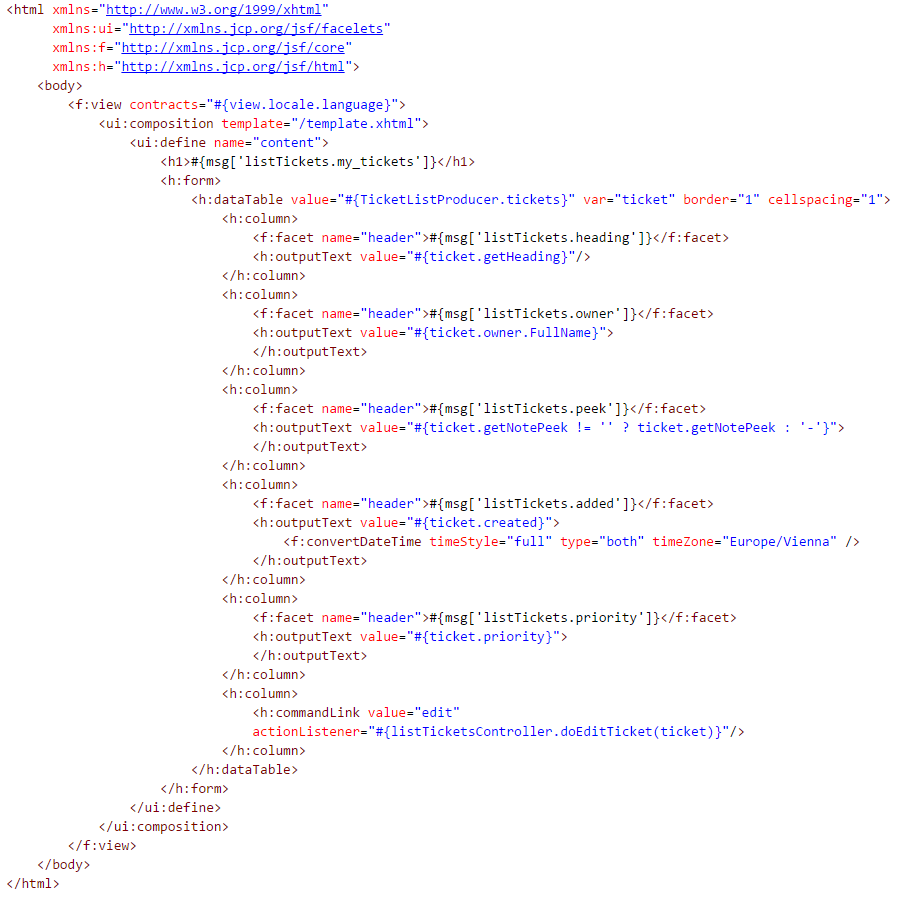
\includegraphics[scale=0.75]{figures/serverFacesCode.png}
	\caption{Ausschnitt JSF XHTML Datei}
	\label{Abb_Jsf_XHTML_Code}
\end{figure}

\newpage
\section{Klassenentwurf}

\begin{figure}[h]
	\centering
	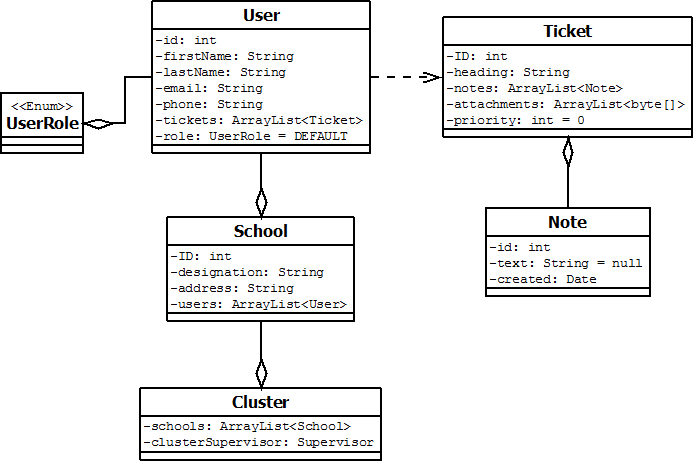
\includegraphics[scale=0.6]{figures/klassenentwurf_java_ticketsys_export.png}
	\caption{Klassenentwurf Java EE Ticketsystem}
	\label{Abb_Klassendesign_TicketSys}
\end{figure}

In Abbildung \ref{Abb_Klassendesign_TicketSys} ist ein simpler Entwurf der Model-Klassen des Ticketsystems als Klassendiagramm dargestellt. Der Benutzer (User) hält Informationen wie deren Namen, Kontaktdetails und eine Liste der vom User erstellten Tickets für die folgenden Rollen:

\begin{description}
	\item[IT Manager bzw. Managerinnen (Managers):] Eine Person an Tirols Schulen, verantwortlich für die lokale Infrastrukturbetreuung und Fehlerreporting
	\item[Systembetreuer bzw. Systembetreuerinnen (Supervisors):] Bearbeitet Meldungen (Tickets) für einen Schulcluster
	\item[Administratoren bzw. Administratorinnen (Admins):] Eine Person des Landesschulrates, verantwortlich für das Gesamtsystem (\getHammerl).
\end{description}

Damit steht die Klasse User im Zentrum des Systems. Die Ticket-Klasse (oder eine Entität des Typs Ticket) hat eine Überschrift, eine Priorität, welche vom User (meist IT Manager(in)) definiert wird, eine Liste an Notes (Fehlerbeschreibungen, Nachrichten in Blogpost-Form) und eine Menge an Dateianhängen.






\section{Sicherheit des Systems}
Beschreibung aller sicherheitsrelevanten Designentscheidungen;

\chapter{Implementierung}
Detaillierte Beschreibung der Implementierung aller Teilkomponenten der Software entlang der zentralsten Use-Cases:

\begin{itemize}
	\item GUI-Implementierung
	\item Controllerlogik
	\item Geschäftslogik
	\item Datenbankzugriffe
\end{itemize}

Detaillierte Beschreibung der Teststrategie (Testdriven Development):

\begin{itemize}
	\item UNIT-Tests (Funktional)
	\item Integrationstests
\end{itemize}

Zu Codesequenzen:
\begin{itemize}
	\item kurze Codesequenzen direkt im Text (mit Zeilnnummern auf die man in der Beschreibung verweisen kann)
	\item lange Codesequenzen in den Anhang (mit Zeilennummer) und darauf verweisen (wie z.B. hier \cref{qj})
\end{itemize}

\chapter{Deployment}
\begin{itemize}
	\item Design der Ausführungsumgebung (Produktivenvironment)
	\item Umsetzung der Ausführungsumgebung
	\item Deployment
	\item DevOps-Thema
\end{itemize}

\chapter{Tests}

%todo: Testfälle doch in diesem Chapter verwenden?!? Vorlage etwas unklar
\section{Systemtests} 
Systemtests aller implementierten Funktionalitäten lt. Pflichtenheft
\begin{itemize}
	\item Beschreibung der Teststrategie
	\item Testfall 1
	\item Testfall 2
	\item Tesfall 3
	\item …
\end{itemize}

\section{Akzeptanztests}

\chapter{Projektevaluation}
siehe Projektmanagement-Unterricht

\chapter{Benutzerhandbuch} 
falls im Projekt gefordert

\chapter{Zusammenfassung}
\begin{itemize}
	\item Etwas längere Form des Abstracts
	\item Detaillierte Beschreibung des Outputs der Arbeit
\end{itemize}